
\clearpage
\subsection{Design 0061}\label{sb:0061}
\noindent\textbf{Verdict: }Admissible (cleaned), rank 1 of 7; smallest reserve 30 \% (σ99 steel 1.4429).\par\smallskip
\begin{minipage}[t]{0.46\linewidth}\small\begin{tabular}[t]{@{}lr@{}}\toprule\multicolumn{2}{@{}l}{\textbf{Design variables}}\\\midrule
coil–plasma distance & \num{0.204} \\
coils in total & 24 \\
coils per half period & \num{6} \\
length per coil & \num{4.58} \\
force weight & \num{0.010} \\
inner wall & \num{0.10} \\
side wall & \num{0.30} \\
outer wall min. & \num{0.52} \\
outer wall extra & \num{0.26} \\
connector stiffness & \num{93} \\
connectors per pair & \num{10} \\
bearing radius & \num{3.23} \\
\bottomrule\end{tabular}\end{minipage}\hfill
\begin{minipage}[t]{0.5\linewidth}\small\begin{tabular}[t]{@{}lr@{}}\toprule\multicolumn{2}{@{}l}{\textbf{Results}}\\\midrule
$\sigma_{99}$ steel 1.4429 & \num{351} MPa \\
largest element & \num{725} MPa \\
$P_m$ max. / 99 \% & \num{522} / \num{379} MPa \\
$P_m+P_b$ max. & \num{938} MPa \\
connectors σ99 & \num{191} MPa \\
max. deformation & \num{18} mm \\
winding-pack strain & \num{0.17} \% \\
current per coil & \num{14.7} MA \\
field at conductor & \num{15.6} T \\
utilisation / margin & \num{30} \% / \num{24} K \\
field error $B\cdot n$ & \num{1.49} ‰ \\
clearance plasma–case & \num{1.62} m \\
nuclear heating / fluence & \num{10} W/m³ / 8.0e16 \\
steel case + connectors & \num{9.5} + \num{9.9} kt \\
connectors built & 236 \\
\bottomrule\end{tabular}\end{minipage}\par\medskip
\noindent\textit{Mesh study ($\sigma_{99}$/max. in MPa): }doe1: 351/725; 1.5× stations: 556/6553; wall 3 cells: 346/861.\par\smallskip
\begin{figure}[H]\centering
\begin{minipage}[t]{0.49\linewidth}\centering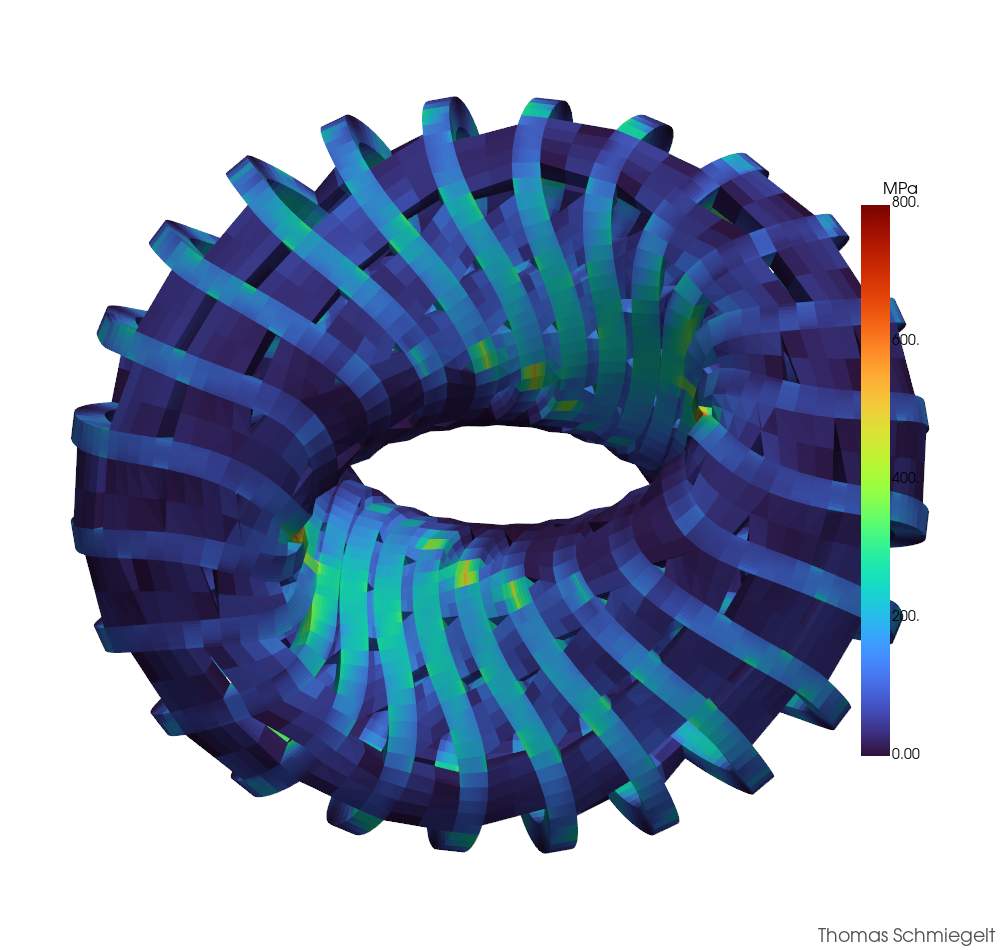
\includegraphics[width=\linewidth]{bilder/spannung_0061.png}\\\footnotesize von Mises stress in the steel (top view, 0–800 MPa)\end{minipage}\hfill
\begin{minipage}[t]{0.49\linewidth}\centering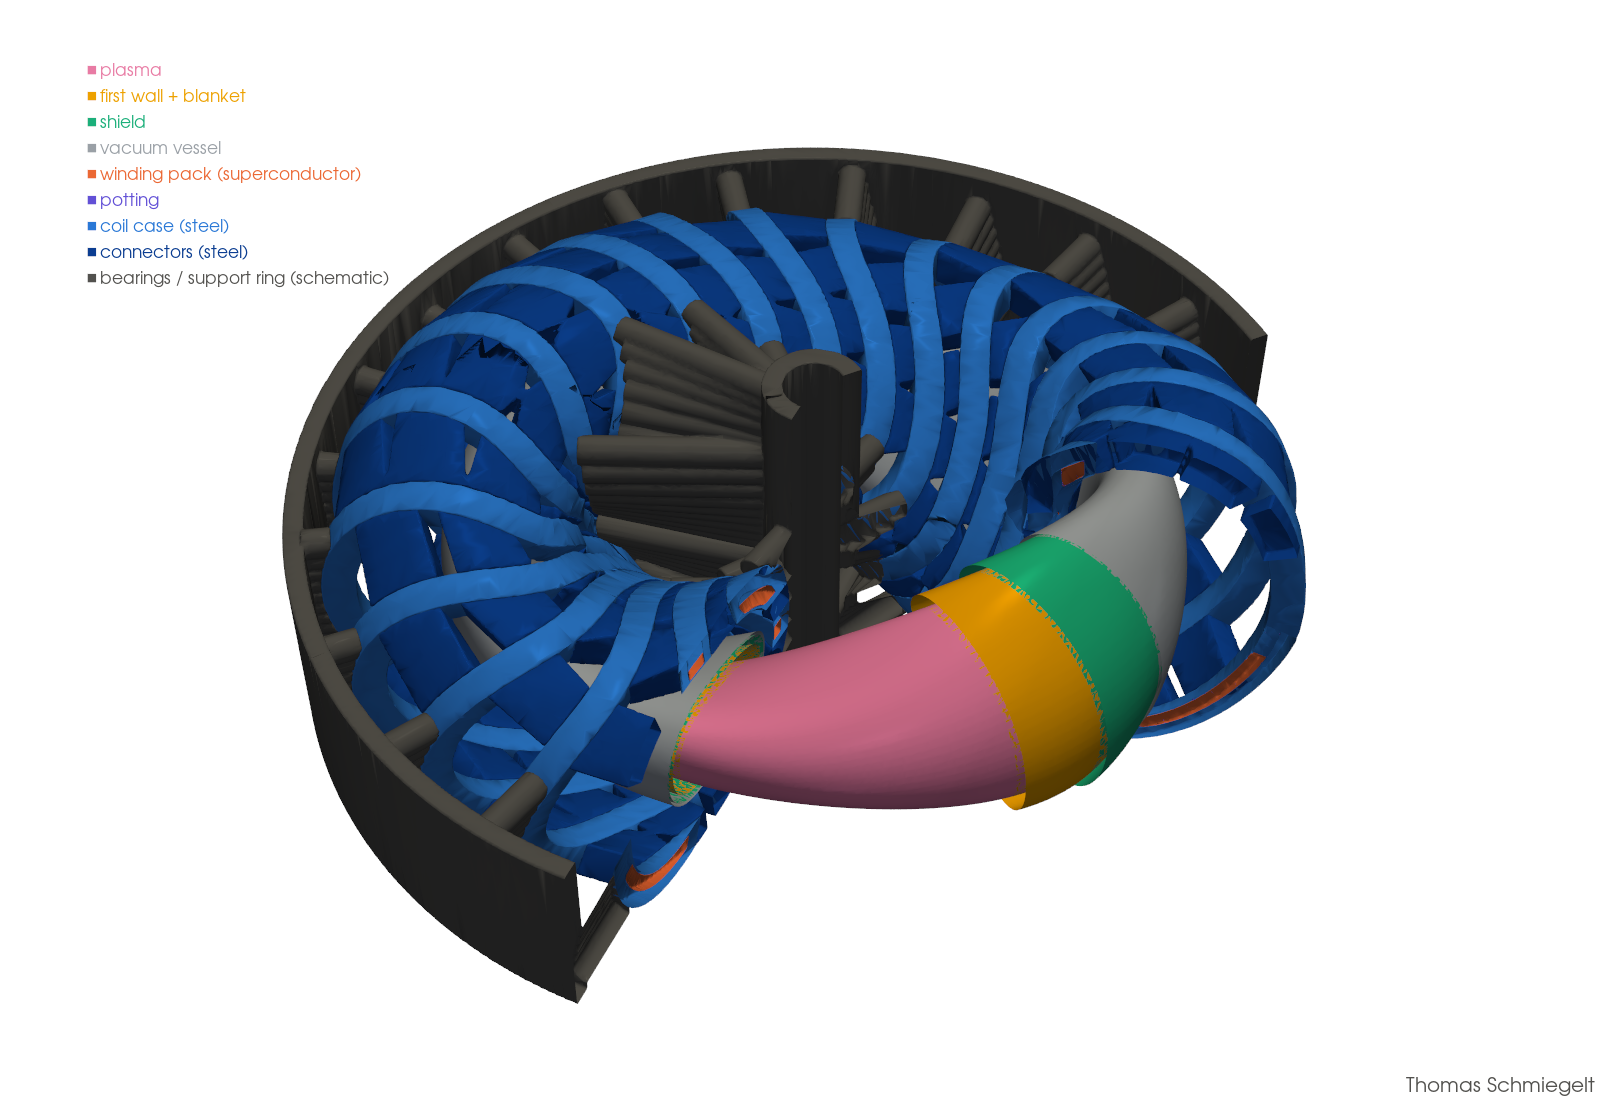
\includegraphics[width=\linewidth]{bilder/modell3d_0061_schnitt_en.png}\\\footnotesize PicoGK model, stepped cut\end{minipage}\hfill
\caption{Design 0061}\end{figure}
\clearpage
\subsection{Design 0169}\label{sb:0169}
\noindent\textbf{Verdict: }Admissible (cleaned), rank 2 of 7; smallest reserve 29 \% (package space).\par\smallskip
\begin{minipage}[t]{0.46\linewidth}\small\begin{tabular}[t]{@{}lr@{}}\toprule\multicolumn{2}{@{}l}{\textbf{Design variables}}\\\midrule
coil–plasma distance & \num{0.197} \\
coils in total & 24 \\
coils per half period & \num{6} \\
length per coil & \num{4.87} \\
force weight & \num{0.023} \\
inner wall & \num{0.27} \\
side wall & \num{0.34} \\
outer wall min. & \num{0.67} \\
outer wall extra & \num{0.25} \\
connector stiffness & \num{183} \\
connectors per pair & \num{13} \\
bearing radius & \num{3.29} \\
\bottomrule\end{tabular}\end{minipage}\hfill
\begin{minipage}[t]{0.5\linewidth}\small\begin{tabular}[t]{@{}lr@{}}\toprule\multicolumn{2}{@{}l}{\textbf{Results}}\\\midrule
$\sigma_{99}$ steel 1.4429 & \num{308} MPa \\
largest element & \num{717} MPa \\
$P_m$ max. / 99 \% & \num{626} / \num{333} MPa \\
$P_m+P_b$ max. & \num{817} MPa \\
connectors σ99 & \num{192} MPa \\
max. deformation & \num{19} mm \\
winding-pack strain & \num{0.15} \% \\
current per coil & \num{14.7} MA \\
field at conductor & \num{15.5} T \\
utilisation / margin & \num{30} \% / \num{24} K \\
field error $B\cdot n$ & \num{2.13} ‰ \\
clearance plasma–case & \num{1.39} m \\
nuclear heating / fluence & \num{103} W/m³ / 8.5e17 \\
steel case + connectors & \num{12.8} + \num{15.2} kt \\
connectors built & 292 \\
\bottomrule\end{tabular}\end{minipage}\par\medskip
\noindent\textit{Mesh study ($\sigma_{99}$/max. in MPa): }doe1: 219/421; standard: 308/717; 1.5× stations: 319/1262; wall 3 cells: 308/794.\par\smallskip
\begin{figure}[H]\centering
\begin{minipage}[t]{0.49\linewidth}\centering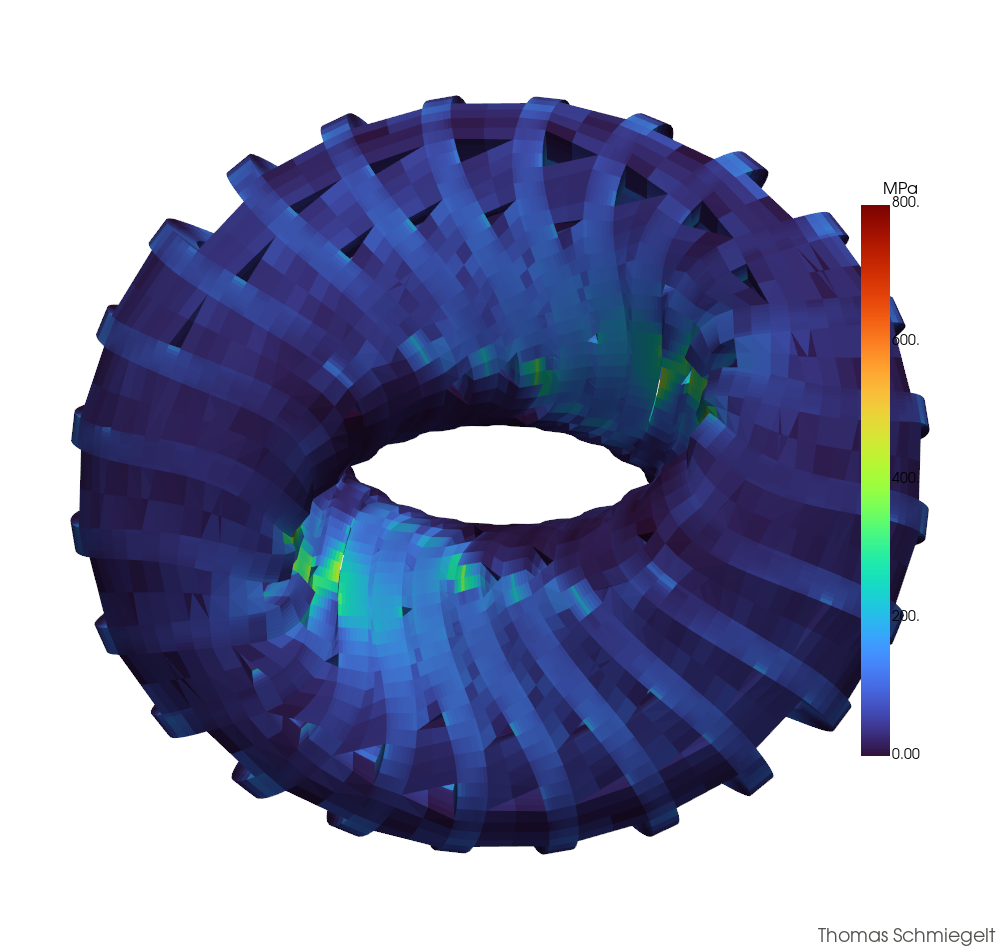
\includegraphics[width=\linewidth]{bilder/spannung_0169.png}\\\footnotesize von Mises stress in the steel (top view, 0–800 MPa)\end{minipage}\hfill
\begin{minipage}[t]{0.49\linewidth}\centering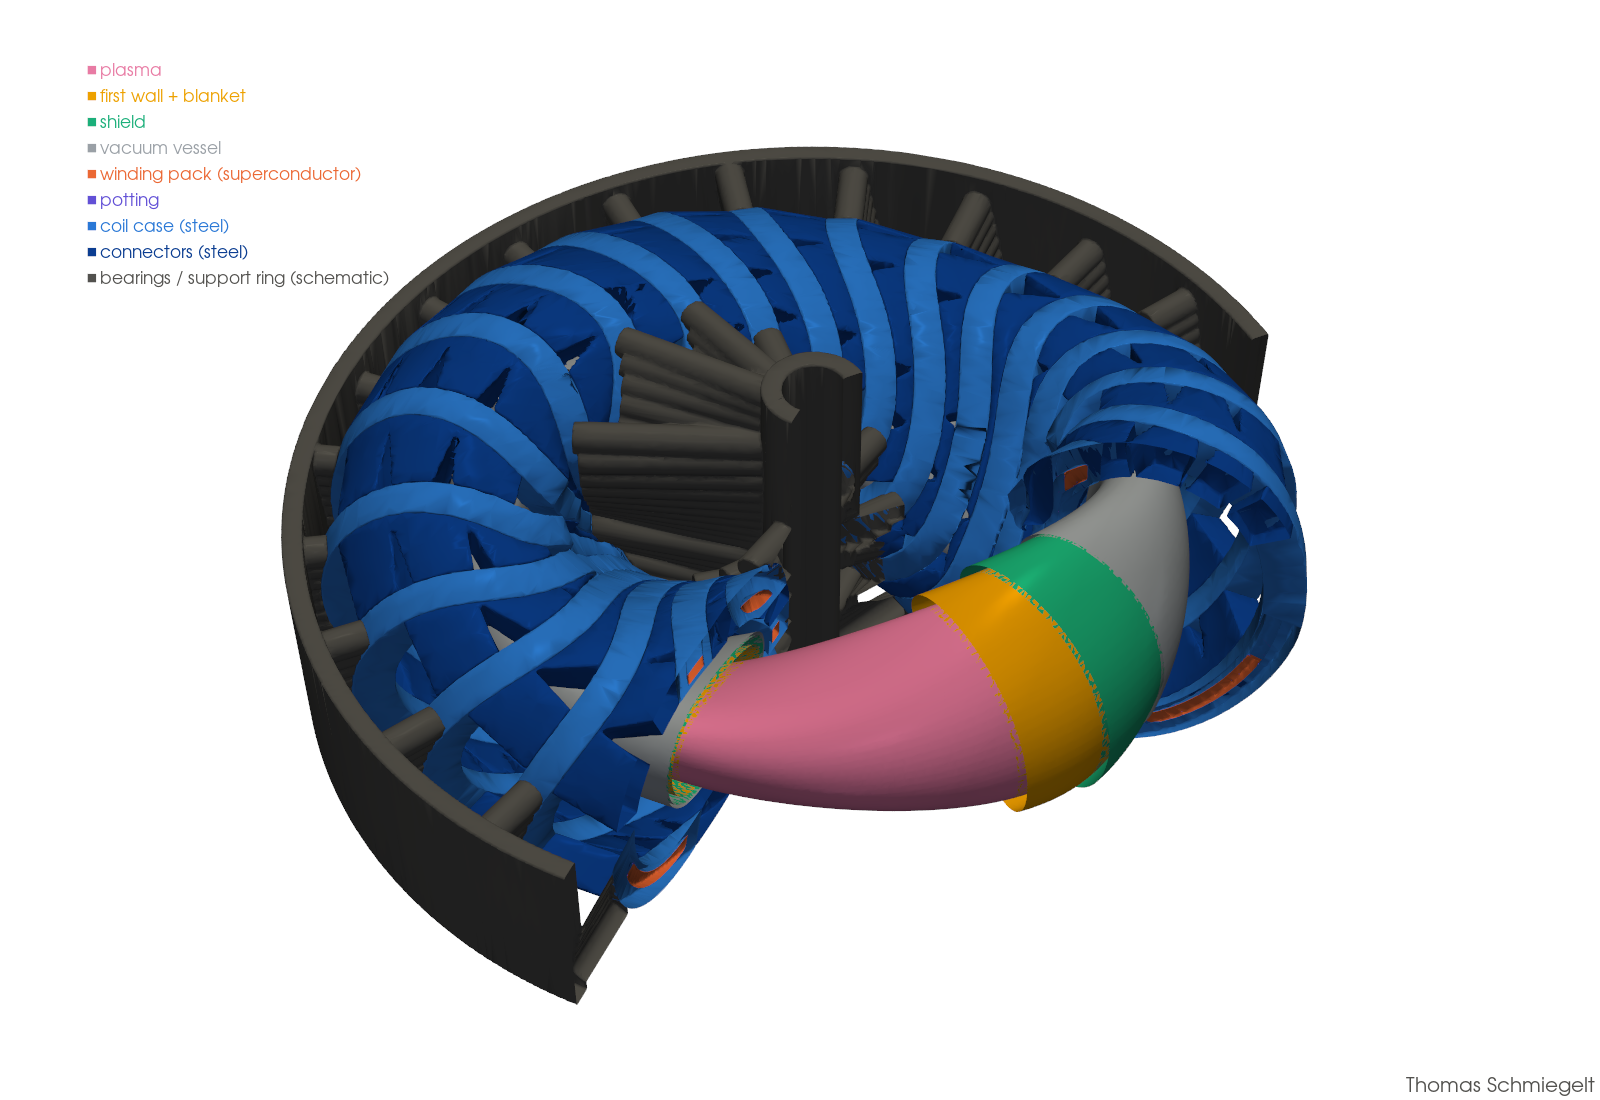
\includegraphics[width=\linewidth]{bilder/modell3d_0169_schnitt_en.png}\\\footnotesize PicoGK model, stepped cut\end{minipage}\hfill
\caption{Design 0169}\end{figure}
\clearpage
\subsection{Design 0093}\label{sb:0093}
\noindent\textbf{Verdict: }Admissible (cleaned), rank 3 of 7; smallest reserve 27 \% (package space).\par\smallskip
\begin{minipage}[t]{0.46\linewidth}\small\begin{tabular}[t]{@{}lr@{}}\toprule\multicolumn{2}{@{}l}{\textbf{Design variables}}\\\midrule
coil–plasma distance & \num{0.206} \\
coils in total & 24 \\
coils per half period & \num{6} \\
length per coil & \num{4.14} \\
force weight & \num{0.010} \\
inner wall & \num{0.38} \\
side wall & \num{0.38} \\
outer wall min. & \num{0.73} \\
outer wall extra & \num{0.38} \\
connector stiffness & \num{64} \\
connectors per pair & \num{8} \\
bearing radius & \num{3.49} \\
\bottomrule\end{tabular}\end{minipage}\hfill
\begin{minipage}[t]{0.5\linewidth}\small\begin{tabular}[t]{@{}lr@{}}\toprule\multicolumn{2}{@{}l}{\textbf{Results}}\\\midrule
$\sigma_{99}$ steel 1.4429 & \num{283} MPa \\
largest element & \num{1190} MPa \\
$P_m$ max. / 99 \% & \num{1147} / \num{340} MPa \\
$P_m+P_b$ max. & \num{1233} MPa \\
connectors σ99 & \num{154} MPa \\
max. deformation & \num{20} mm \\
winding-pack strain & \num{0.16} \% \\
current per coil & \num{14.7} MA \\
field at conductor & \num{15.7} T \\
utilisation / margin & \num{30} \% / \num{24} K \\
field error $B\cdot n$ & \num{1.45} ‰ \\
clearance plasma–case & \num{1.37} m \\
nuclear heating / fluence & \num{117} W/m³ / 9.8e17 \\
steel case + connectors & \num{16.5} + \num{11.6} kt \\
connectors built & 190 \\
\bottomrule\end{tabular}\end{minipage}\par\medskip
\noindent\textit{Mesh study ($\sigma_{99}$/max. in MPa): }doe1: 283/1190; 1.5× stations: 410/2343; wall 3 cells: 280/1432.\par\smallskip
\begin{figure}[H]\centering
\begin{minipage}[t]{0.49\linewidth}\centering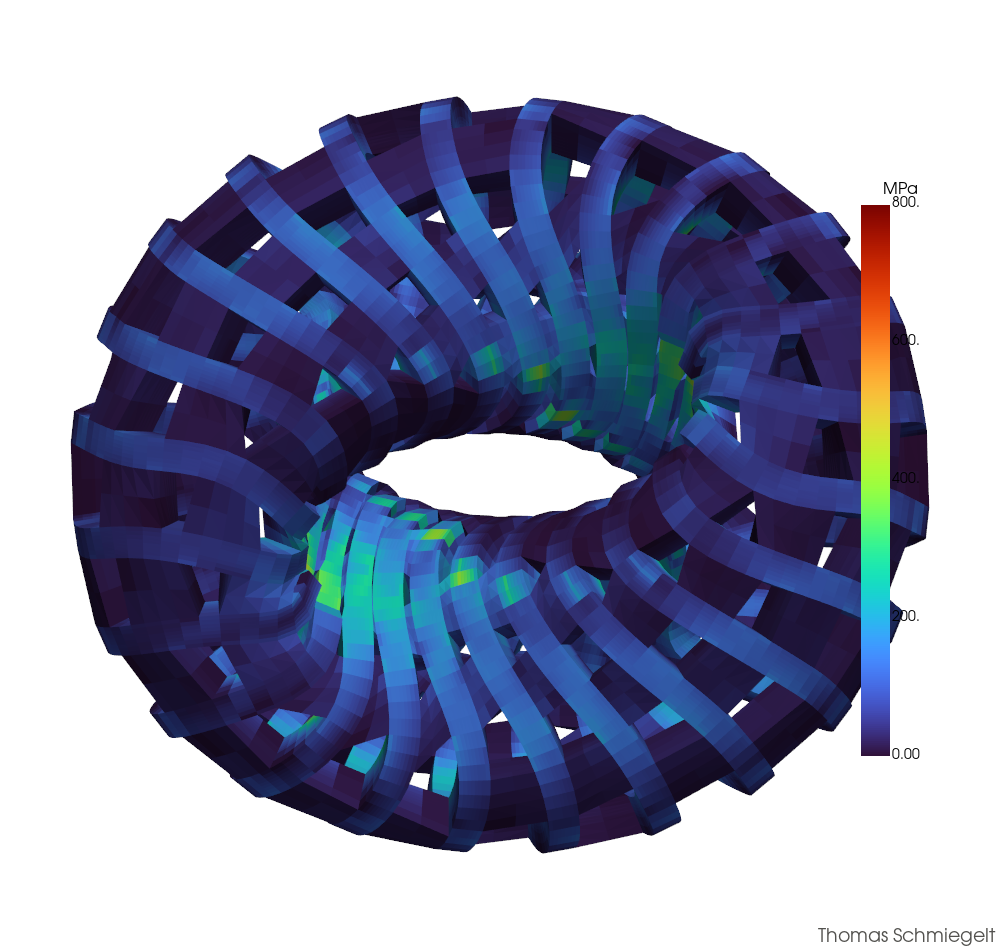
\includegraphics[width=\linewidth]{bilder/spannung_0093.png}\\\footnotesize von Mises stress in the steel (top view, 0–800 MPa)\end{minipage}\hfill
\begin{minipage}[t]{0.49\linewidth}\centering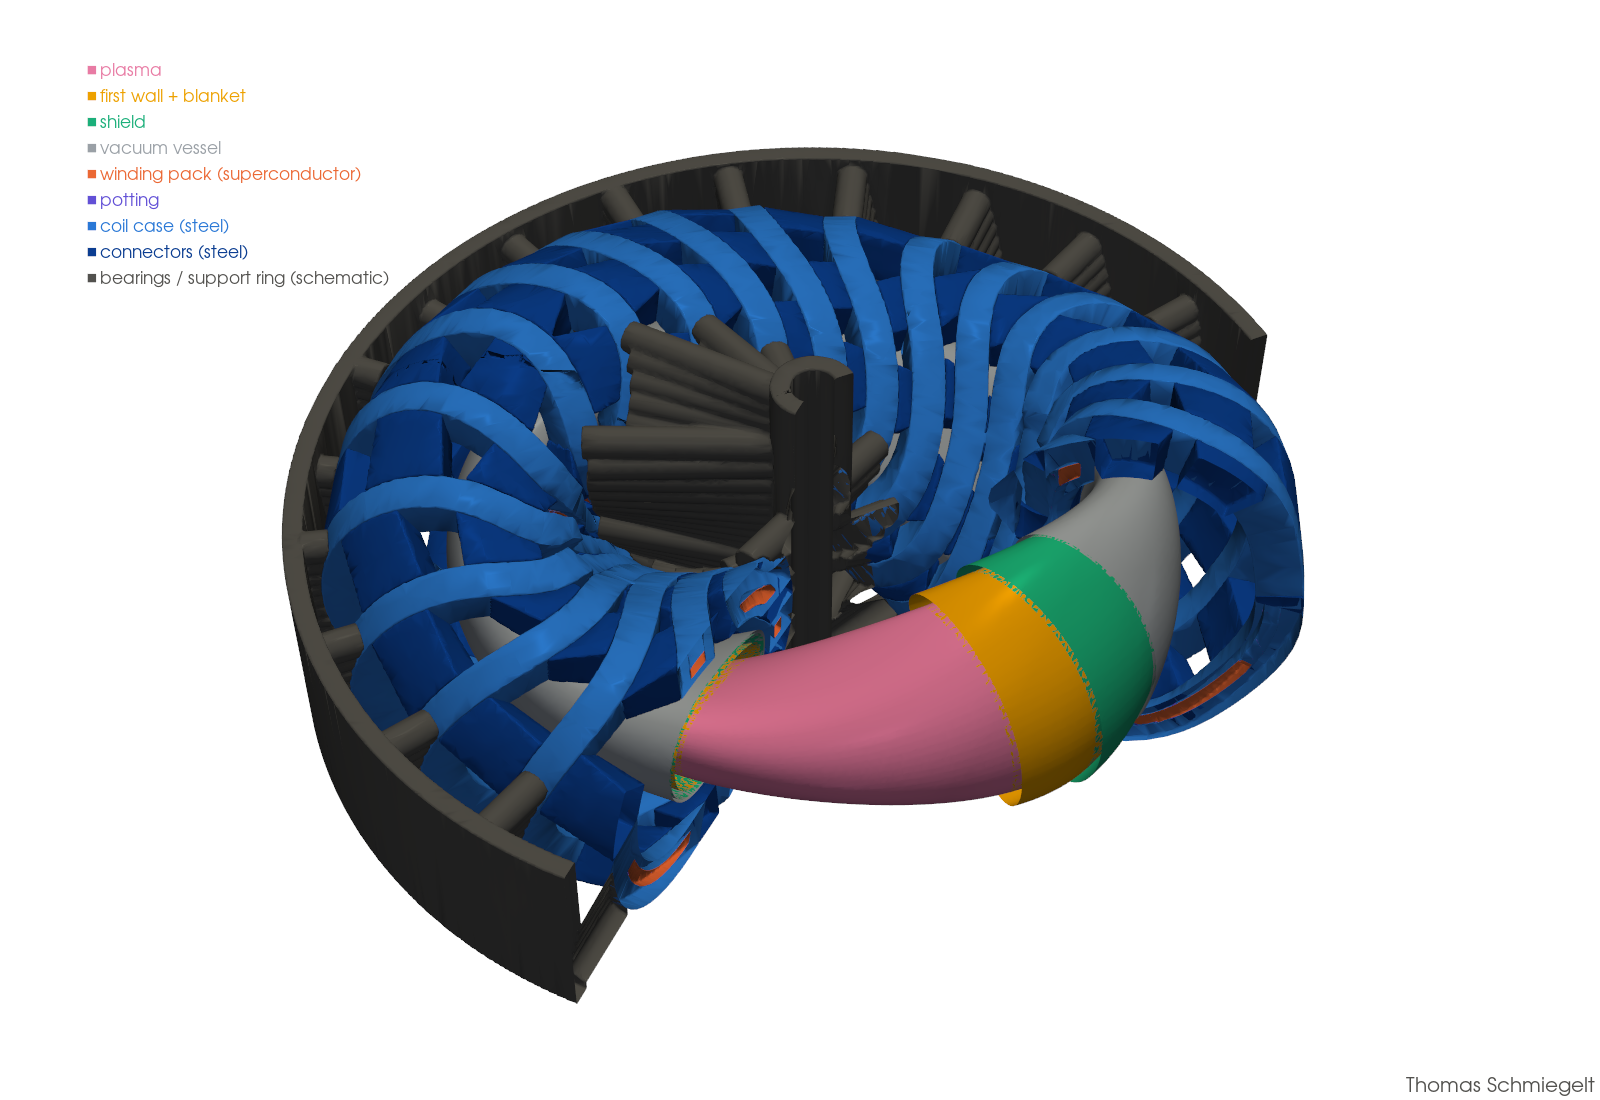
\includegraphics[width=\linewidth]{bilder/modell3d_0093_schnitt_en.png}\\\footnotesize PicoGK model, stepped cut\end{minipage}\hfill
\caption{Design 0093}\end{figure}
\clearpage
\subsection{Design 0008}\label{sb:0008}
\noindent\textbf{Verdict: }Admissible (cleaned), rank 4 of 7; smallest reserve 27 \% (field error B·n).\par\smallskip
\begin{minipage}[t]{0.46\linewidth}\small\begin{tabular}[t]{@{}lr@{}}\toprule\multicolumn{2}{@{}l}{\textbf{Design variables}}\\\midrule
coil–plasma distance & \num{0.211} \\
coils in total & 24 \\
coils per half period & \num{6} \\
length per coil & \num{3.66} \\
force weight & \num{0.030} \\
inner wall & \num{0.32} \\
side wall & \num{0.31} \\
outer wall min. & \num{0.72} \\
outer wall extra & \num{0.17} \\
connector stiffness & \num{142} \\
connectors per pair & \num{11} \\
bearing radius & \num{2.80} \\
\bottomrule\end{tabular}\end{minipage}\hfill
\begin{minipage}[t]{0.5\linewidth}\small\begin{tabular}[t]{@{}lr@{}}\toprule\multicolumn{2}{@{}l}{\textbf{Results}}\\\midrule
$\sigma_{99}$ steel 1.4429 & \num{305} MPa \\
largest element & \num{1695} MPa \\
$P_m$ max. / 99 \% & \num{1687} / \num{344} MPa \\
$P_m+P_b$ max. & \num{1704} MPa \\
connectors σ99 & \num{187} MPa \\
max. deformation & \num{19} mm \\
winding-pack strain & \num{0.17} \% \\
current per coil & \num{14.7} MA \\
field at conductor & \num{15.7} T \\
utilisation / margin & \num{30} \% / \num{24} K \\
field error $B\cdot n$ & \num{2.20} ‰ \\
clearance plasma–case & \num{1.48} m \\
nuclear heating / fluence & \num{40} W/m³ / 3.3e17 \\
steel case + connectors & \num{12.2} + \num{13.7} kt \\
connectors built & 252 \\
\bottomrule\end{tabular}\end{minipage}\par\medskip
\noindent\textit{Mesh study ($\sigma_{99}$/max. in MPa): }doe1: 305/1695; 1.5× stations: 407/3250; wall 3 cells: 306/1931.\par\smallskip
\begin{figure}[H]\centering
\begin{minipage}[t]{0.49\linewidth}\centering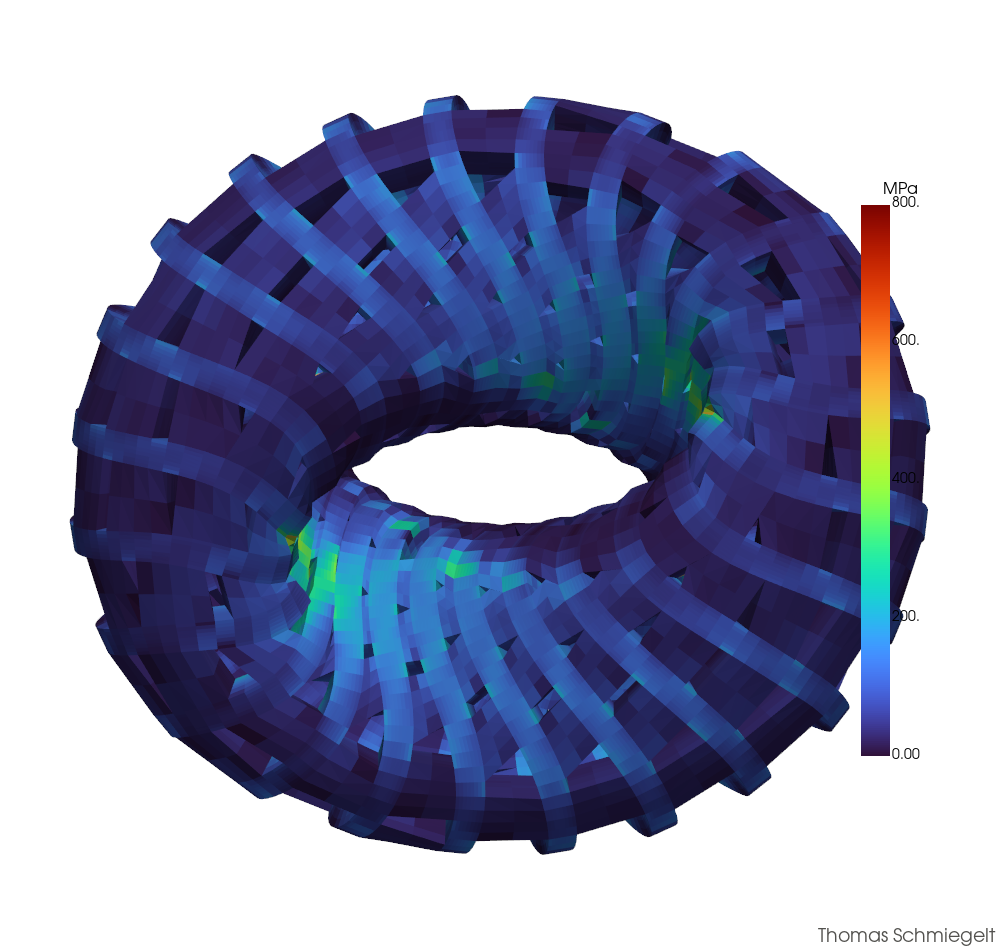
\includegraphics[width=\linewidth]{bilder/spannung_0008.png}\\\footnotesize von Mises stress in the steel (top view, 0–800 MPa)\end{minipage}\hfill
\begin{minipage}[t]{0.49\linewidth}\centering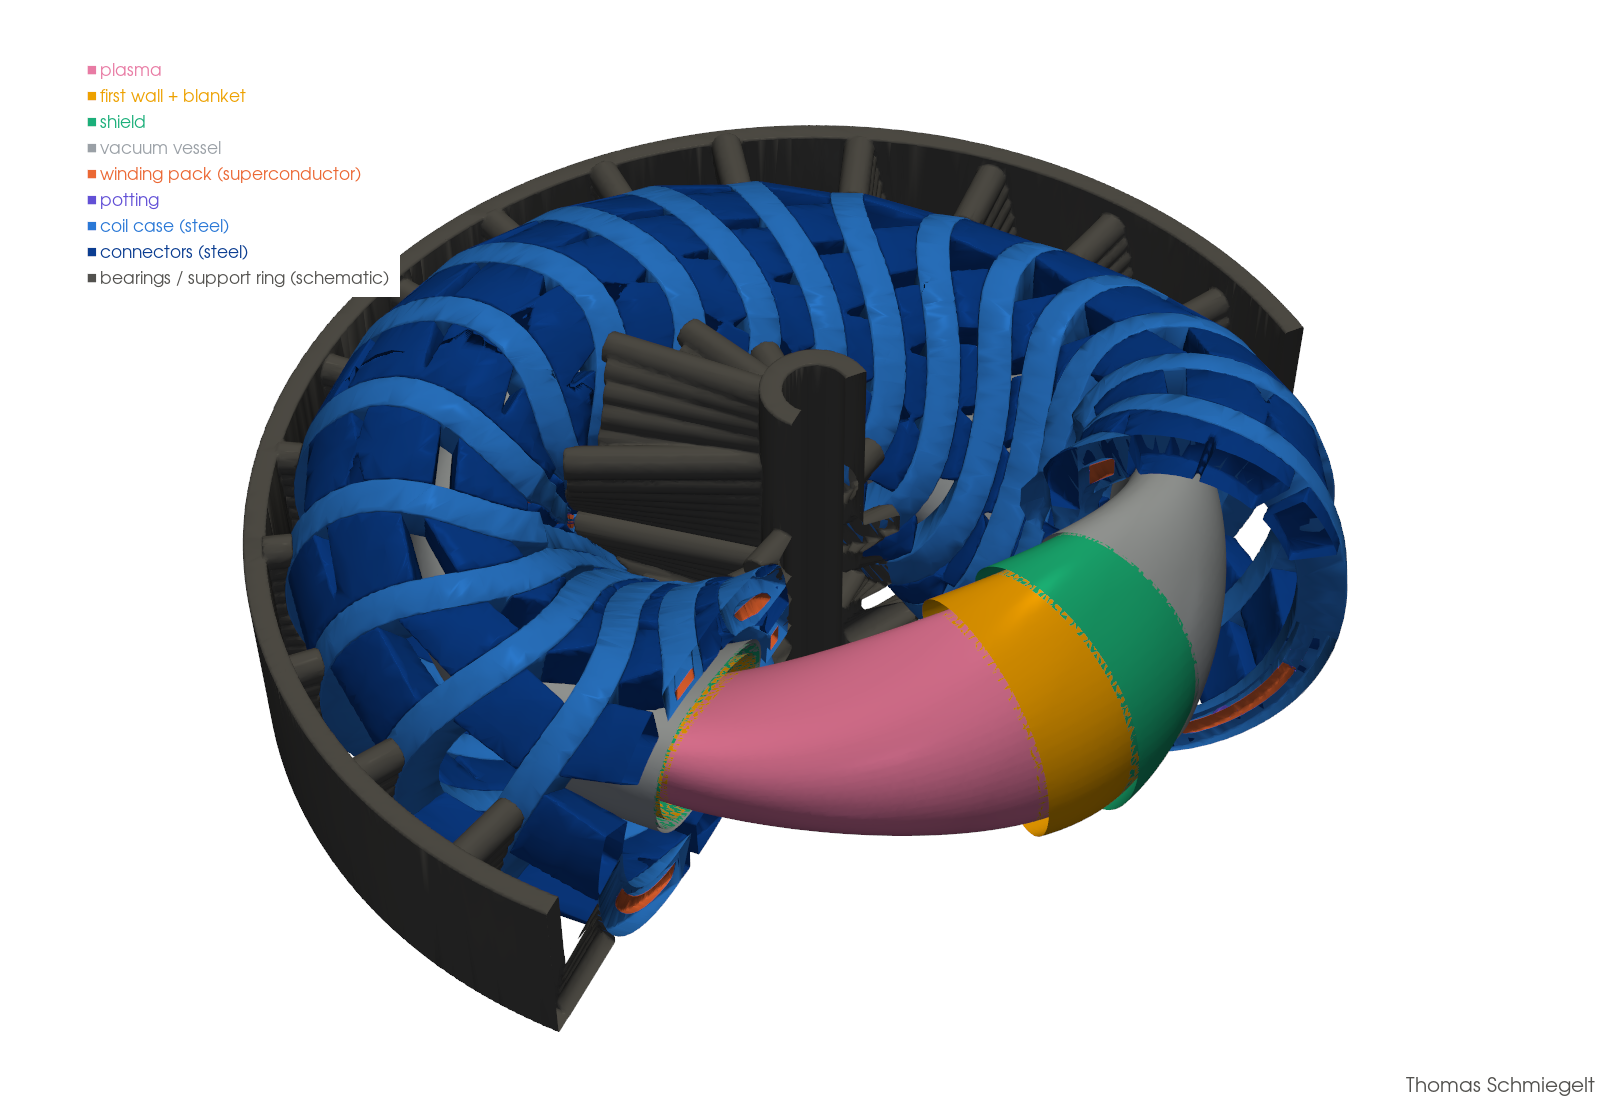
\includegraphics[width=\linewidth]{bilder/modell3d_0008_schnitt_en.png}\\\footnotesize PicoGK model, stepped cut\end{minipage}\hfill
\caption{Design 0008}\end{figure}
\clearpage
\subsection{Design 0014}\label{sb:0014}
\noindent\textbf{Verdict: }Admissible (cleaned), rank 5 of 7; smallest reserve 25 \% (σ99 steel 1.4429).\par\smallskip
\begin{minipage}[t]{0.46\linewidth}\small\begin{tabular}[t]{@{}lr@{}}\toprule\multicolumn{2}{@{}l}{\textbf{Design variables}}\\\midrule
coil–plasma distance & \num{0.233} \\
coils in total & 20 \\
coils per half period & \num{5} \\
length per coil & \num{4.34} \\
force weight & \num{0.025} \\
inner wall & \num{0.35} \\
side wall & \num{0.32} \\
outer wall min. & \num{0.63} \\
outer wall extra & \num{0.29} \\
connector stiffness & \num{196} \\
connectors per pair & \num{11} \\
bearing radius & \num{2.04} \\
\bottomrule\end{tabular}\end{minipage}\hfill
\begin{minipage}[t]{0.5\linewidth}\small\begin{tabular}[t]{@{}lr@{}}\toprule\multicolumn{2}{@{}l}{\textbf{Results}}\\\midrule
$\sigma_{99}$ steel 1.4429 & \num{377} MPa \\
largest element & \num{1419} MPa \\
$P_m$ max. / 99 \% & \num{1369} / \num{459} MPa \\
$P_m+P_b$ max. & \num{1491} MPa \\
connectors σ99 & \num{243} MPa \\
max. deformation & \num{18} mm \\
winding-pack strain & \num{0.21} \% \\
current per coil & \num{17.7} MA \\
field at conductor & \num{16.9} T \\
utilisation / margin & \num{32} \% / \num{23} K \\
field error $B\cdot n$ & \num{2.21} ‰ \\
clearance plasma–case & \num{1.65} m \\
nuclear heating / fluence & \num{8} W/m³ / 6.5e16 \\
steel case + connectors & \num{12.5} + \num{15.5} kt \\
connectors built & 212 \\
\bottomrule\end{tabular}\end{minipage}\par\medskip
\noindent\textit{Mesh study ($\sigma_{99}$/max. in MPa): }doe1: 377/1419; 1.5× stations: 549/3814; wall 3 cells: 375/1639.\par\smallskip
\begin{figure}[H]\centering
\begin{minipage}[t]{0.49\linewidth}\centering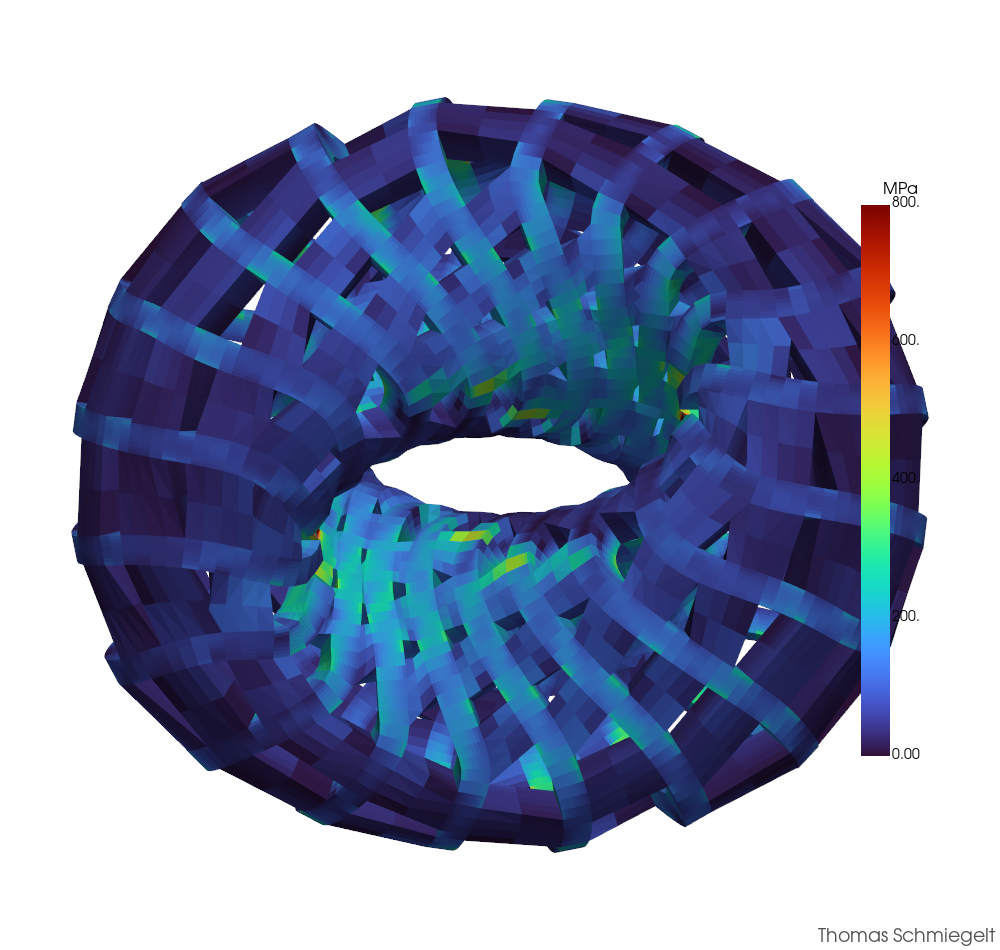
\includegraphics[width=\linewidth]{bilder/spannung_0014.png}\\\footnotesize von Mises stress in the steel (top view, 0–800 MPa)\end{minipage}\hfill
\begin{minipage}[t]{0.49\linewidth}\centering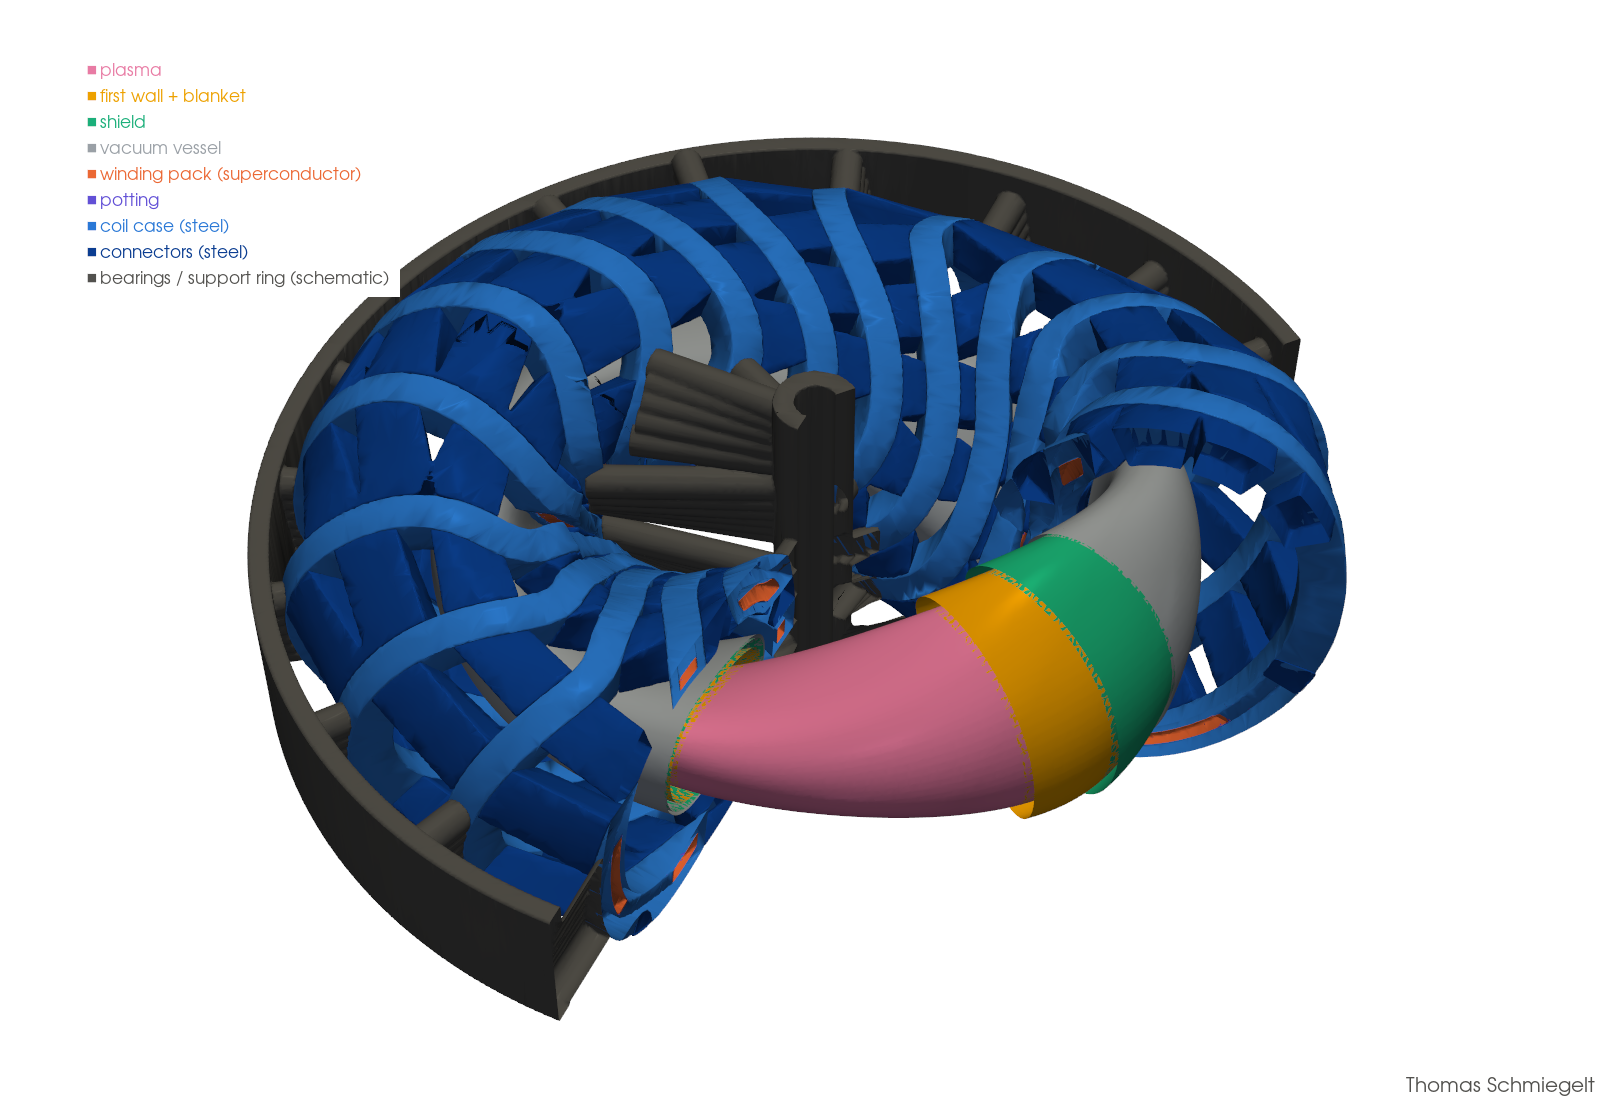
\includegraphics[width=\linewidth]{bilder/modell3d_0014_schnitt_en.png}\\\footnotesize PicoGK model, stepped cut\end{minipage}\hfill
\caption{Design 0014}\end{figure}
\clearpage
\subsection{Design 0017}\label{sb:0017}
\noindent\textbf{Verdict: }Admissible (cleaned), rank 6 of 7; smallest reserve 20 \% (package space).\par\smallskip
\begin{minipage}[t]{0.46\linewidth}\small\begin{tabular}[t]{@{}lr@{}}\toprule\multicolumn{2}{@{}l}{\textbf{Design variables}}\\\midrule
coil–plasma distance & \num{0.220} \\
coils in total & 24 \\
coils per half period & \num{6} \\
length per coil & \num{3.77} \\
force weight & \num{0.019} \\
inner wall & \num{0.60} \\
side wall & \num{0.37} \\
outer wall min. & \num{0.43} \\
outer wall extra & \num{0.32} \\
connector stiffness & \num{29} \\
connectors per pair & \num{7} \\
bearing radius & \num{3.47} \\
\bottomrule\end{tabular}\end{minipage}\hfill
\begin{minipage}[t]{0.5\linewidth}\small\begin{tabular}[t]{@{}lr@{}}\toprule\multicolumn{2}{@{}l}{\textbf{Results}}\\\midrule
$\sigma_{99}$ steel 1.4429 & \num{389} MPa \\
largest element & \num{1721} MPa \\
$P_m$ max. / 99 \% & \num{1631} / \num{448} MPa \\
$P_m+P_b$ max. & \num{1813} MPa \\
connectors σ99 & \num{131} MPa \\
max. deformation & \num{31} mm \\
winding-pack strain & \num{0.20} \% \\
current per coil & \num{14.7} MA \\
field at conductor & \num{16.0} T \\
utilisation / margin & \num{30} \% / \num{24} K \\
field error $B\cdot n$ & \num{1.66} ‰ \\
clearance plasma–case & \num{1.30} m \\
nuclear heating / fluence & \num{245} W/m³ / 2.0e18 \\
steel case + connectors & \num{13.9} + \num{8.7} kt \\
connectors built & 162 \\
\bottomrule\end{tabular}\end{minipage}\par\medskip
\begin{figure}[H]\centering
\begin{minipage}[t]{0.49\linewidth}\centering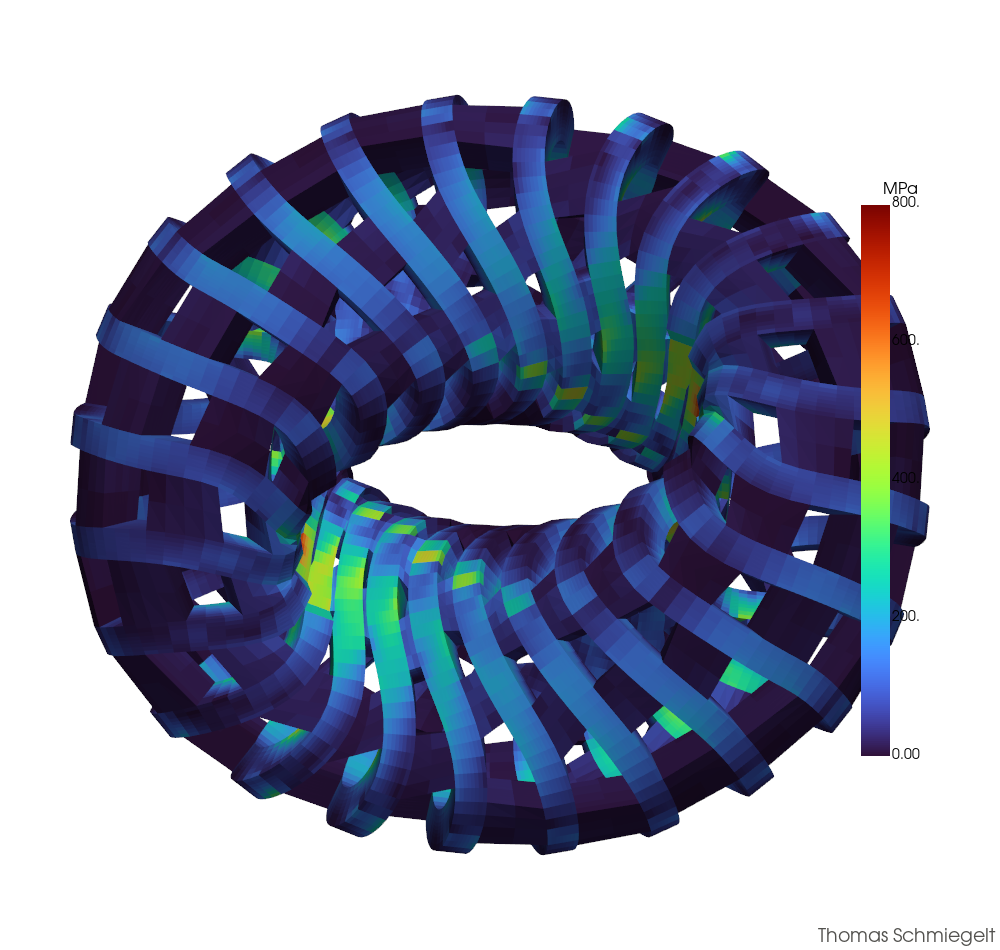
\includegraphics[width=\linewidth]{bilder/spannung_0017.png}\\\footnotesize von Mises stress in the steel (top view, 0–800 MPa)\end{minipage}\hfill
\begin{minipage}[t]{0.49\linewidth}\centering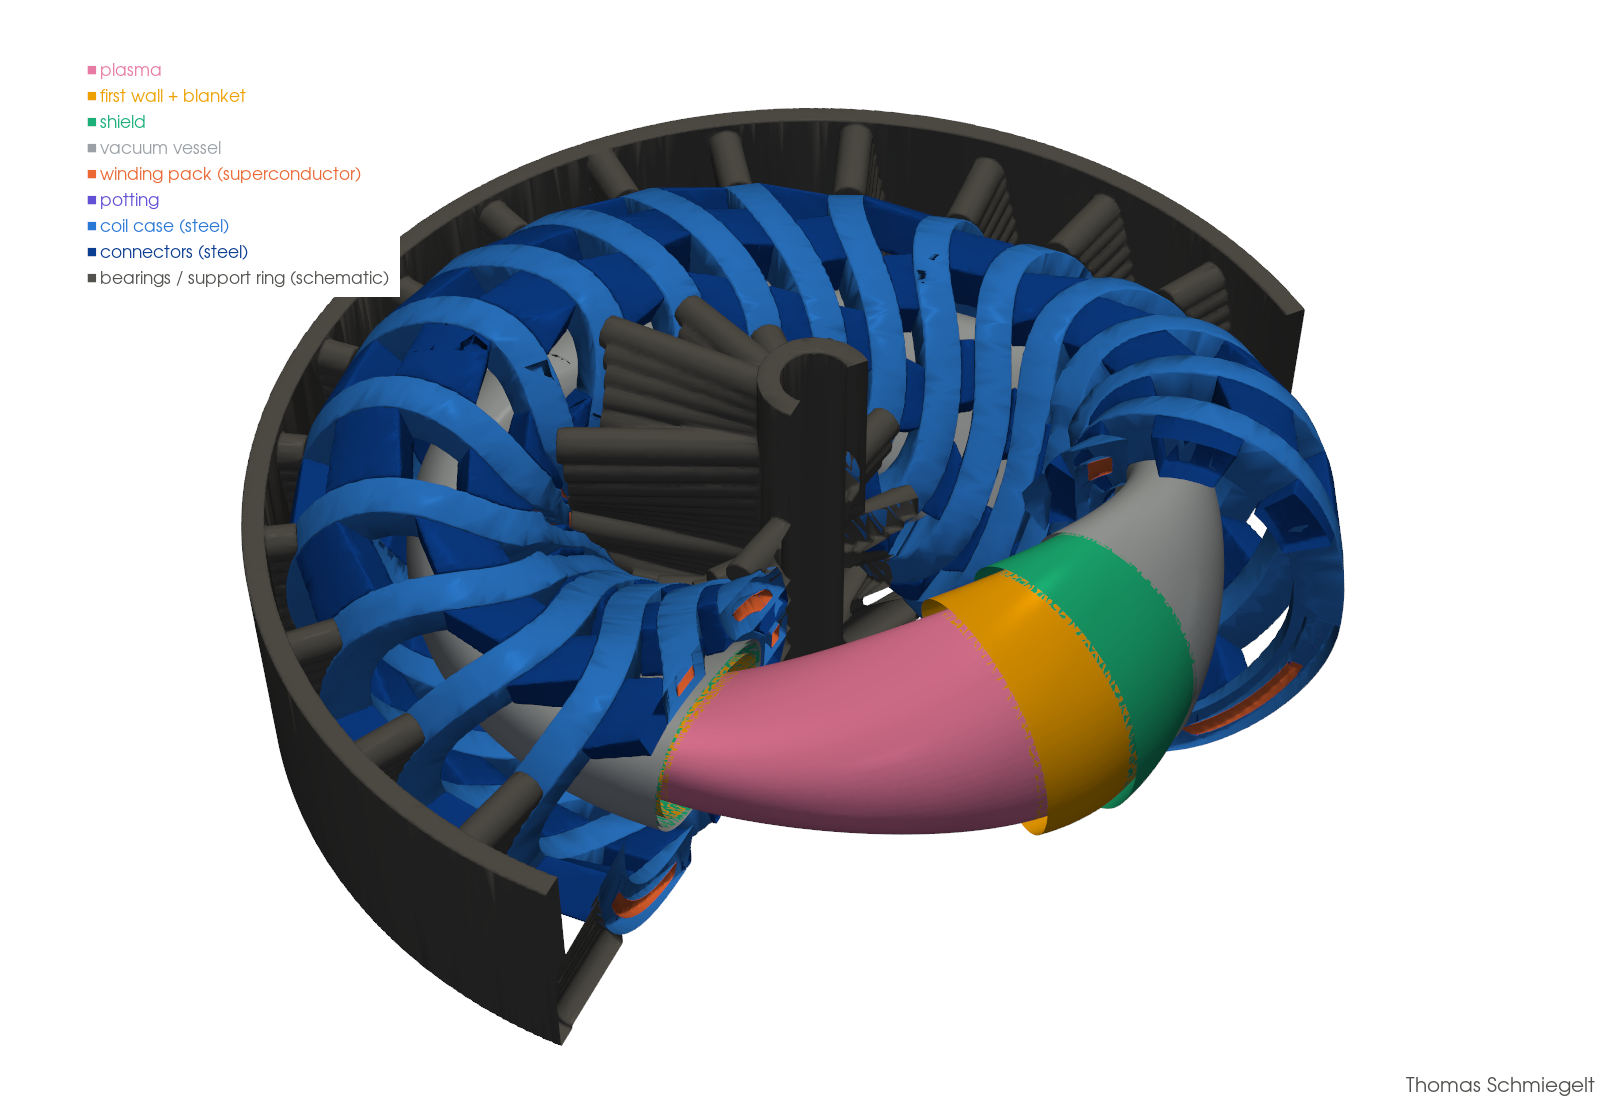
\includegraphics[width=\linewidth]{bilder/modell3d_0017_schnitt_en.png}\\\footnotesize PicoGK model, stepped cut\end{minipage}\hfill
\caption{Design 0017}\end{figure}
\clearpage
\subsection{Design 0157}\label{sb:0157}
\noindent\textbf{Verdict: }Admissible (cleaned), rank 7 of 7; smallest reserve 2 \% (σ99 steel 1.4429).\par\smallskip
\begin{minipage}[t]{0.46\linewidth}\small\begin{tabular}[t]{@{}lr@{}}\toprule\multicolumn{2}{@{}l}{\textbf{Design variables}}\\\midrule
coil–plasma distance & \num{0.218} \\
coils in total & 20 \\
coils per half period & \num{5} \\
length per coil & \num{4.09} \\
force weight & \num{0.020} \\
inner wall & \num{0.49} \\
side wall & \num{0.25} \\
outer wall min. & \num{0.58} \\
outer wall extra & \num{0.02} \\
connector stiffness & \num{158} \\
connectors per pair & \num{6} \\
bearing radius & \num{3.06} \\
\bottomrule\end{tabular}\end{minipage}\hfill
\begin{minipage}[t]{0.5\linewidth}\small\begin{tabular}[t]{@{}lr@{}}\toprule\multicolumn{2}{@{}l}{\textbf{Results}}\\\midrule
$\sigma_{99}$ steel 1.4429 & \num{492} MPa \\
largest element & \num{1658} MPa \\
$P_m$ max. / 99 \% & \num{1405} / \num{519} MPa \\
$P_m+P_b$ max. & \num{1920} MPa \\
connectors σ99 & \num{335} MPa \\
max. deformation & \num{34} mm \\
winding-pack strain & \num{0.22} \% \\
current per coil & \num{17.7} MA \\
field at conductor & \num{16.5} T \\
utilisation / margin & \num{31} \% / \num{23} K \\
field error $B\cdot n$ & \num{2.37} ‰ \\
clearance plasma–case & \num{1.35} m \\
nuclear heating / fluence & \num{142} W/m³ / 1.2e18 \\
steel case + connectors & \num{10.1} + \num{7.5} kt \\
connectors built & 118 \\
\bottomrule\end{tabular}\end{minipage}\par\medskip
\begin{figure}[H]\centering
\begin{minipage}[t]{0.49\linewidth}\centering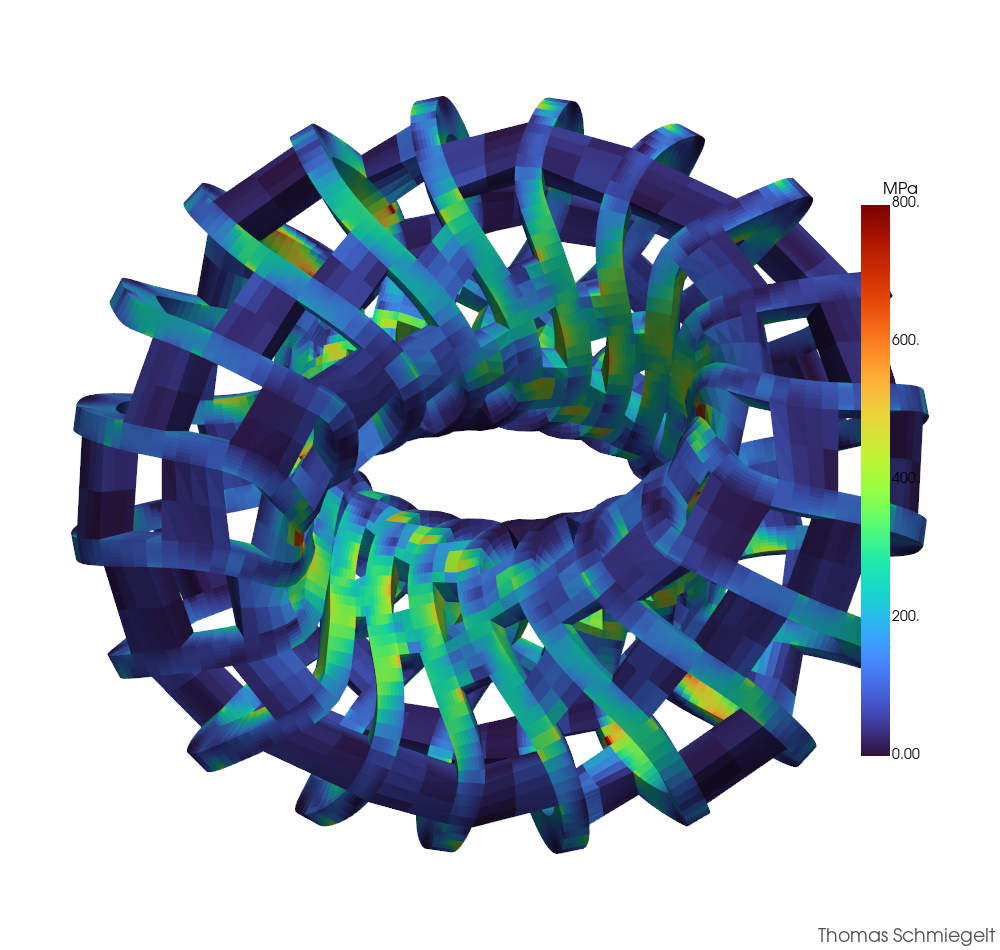
\includegraphics[width=\linewidth]{bilder/spannung_0157.png}\\\footnotesize von Mises stress in the steel (top view, 0–800 MPa)\end{minipage}\hfill
\begin{minipage}[t]{0.49\linewidth}\centering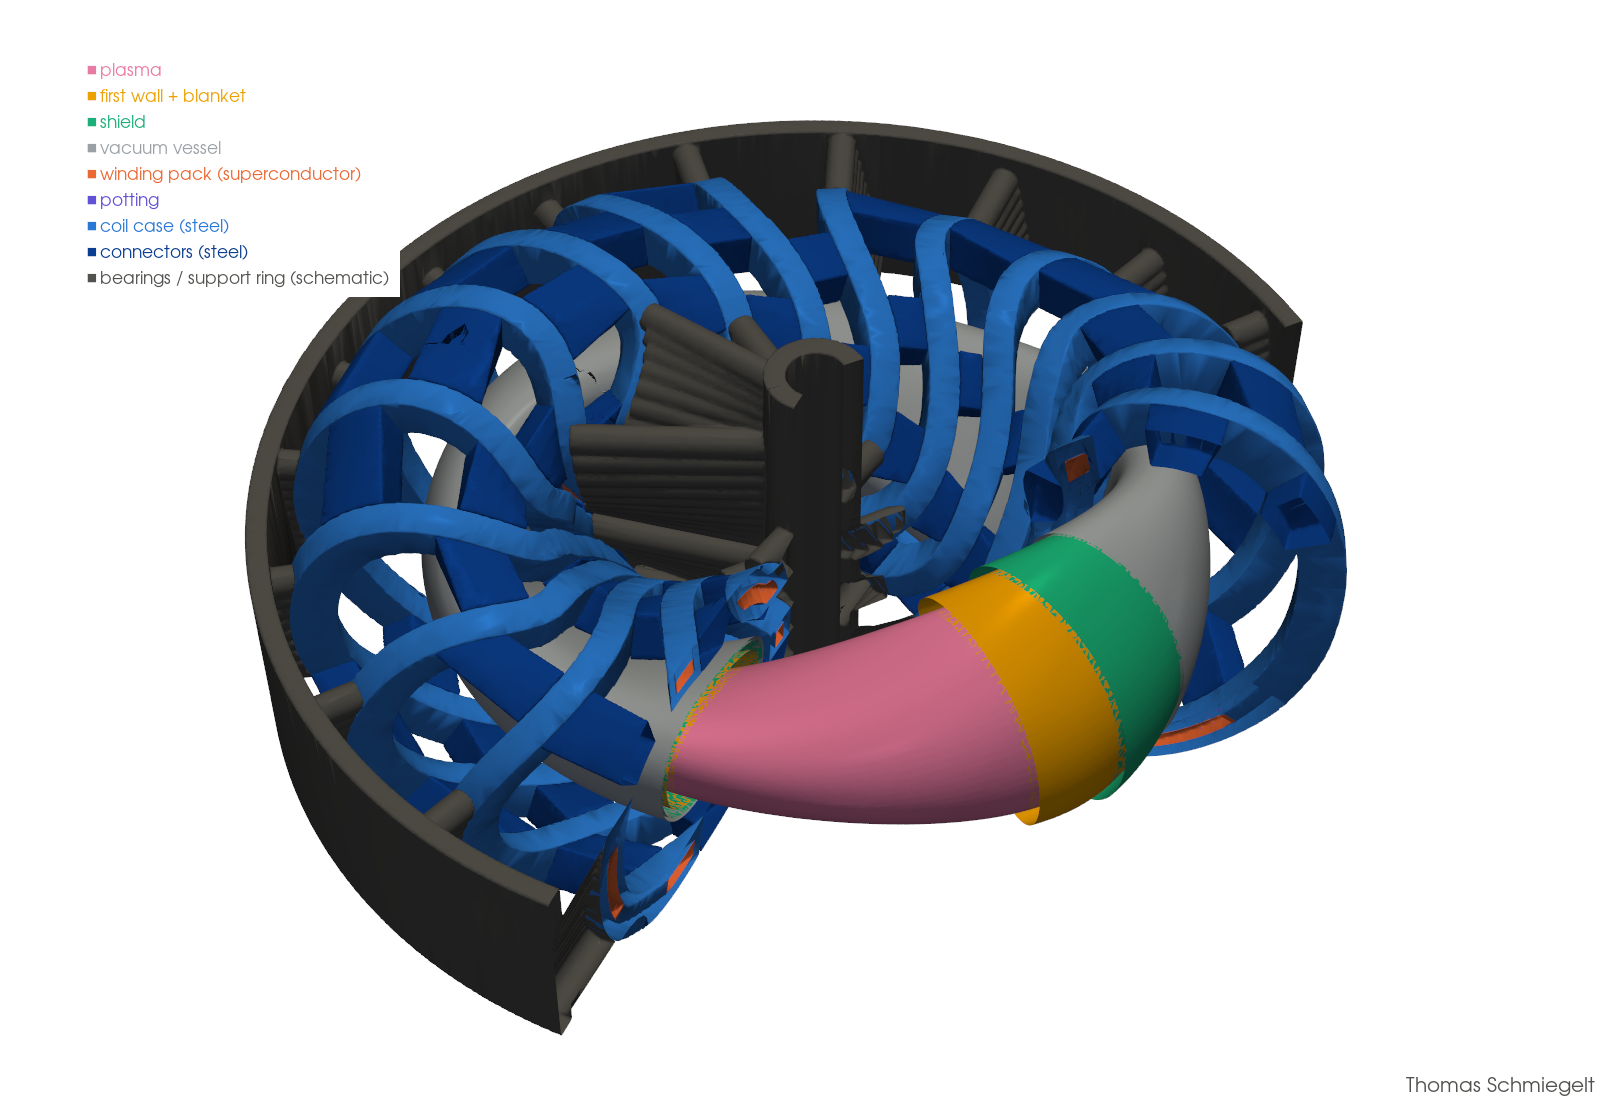
\includegraphics[width=\linewidth]{bilder/modell3d_0157_schnitt_en.png}\\\footnotesize PicoGK model, stepped cut\end{minipage}\hfill
\caption{Design 0157}\end{figure}
\clearpage
\subsection{Design 0063}\label{sb:0063}
\noindent\textbf{Verdict: }Admissible in doe1, no longer with the standard mesh: bottleneck winding-pack strain (reserve -24 \%).\par\smallskip
\begin{minipage}[t]{0.46\linewidth}\small\begin{tabular}[t]{@{}lr@{}}\toprule\multicolumn{2}{@{}l}{\textbf{Design variables}}\\\midrule
coil–plasma distance & \num{0.177} \\
coils in total & 20 \\
coils per half period & \num{5} \\
length per coil & \num{4.45} \\
force weight & \num{0.000} \\
inner wall & \num{0.59} \\
side wall & \num{0.35} \\
outer wall min. & \num{0.69} \\
outer wall extra & \num{0.44} \\
connector stiffness & \num{43} \\
connectors per pair & \num{14} \\
bearing radius & \num{1.71} \\
\bottomrule\end{tabular}\end{minipage}\hfill
\begin{minipage}[t]{0.5\linewidth}\small\begin{tabular}[t]{@{}lr@{}}\toprule\multicolumn{2}{@{}l}{\textbf{Results}}\\\midrule
$\sigma_{99}$ steel 1.4429 & \num{595} MPa \\
largest element & \num{4265} MPa \\
$P_m$ max. / 99 \% & \num{4261} / \num{942} MPa \\
$P_m+P_b$ max. & \num{4270} MPa \\
connectors σ99 & \num{200} MPa \\
max. deformation & \num{81} mm \\
winding-pack strain & \num{0.37} \% \\
current per coil & \num{17.7} MA \\
field at conductor & \num{17.5} T \\
utilisation / margin & \num{33} \% / \num{22} K \\
field error $B\cdot n$ & \num{0.75} ‰ \\
clearance plasma–case & \num{1.53} m \\
nuclear heating / fluence & \num{24} W/m³ / 2.0e17 \\
steel case + connectors & \num{16.7} + \num{24.2} kt \\
connectors built & 252 \\
\bottomrule\end{tabular}\end{minipage}\par\medskip
\noindent\textit{Mesh study ($\sigma_{99}$/max. in MPa): }doe1: 369/2016; standard: 595/4265.\par\smallskip
\begin{figure}[H]\centering
\begin{minipage}[t]{0.49\linewidth}\centering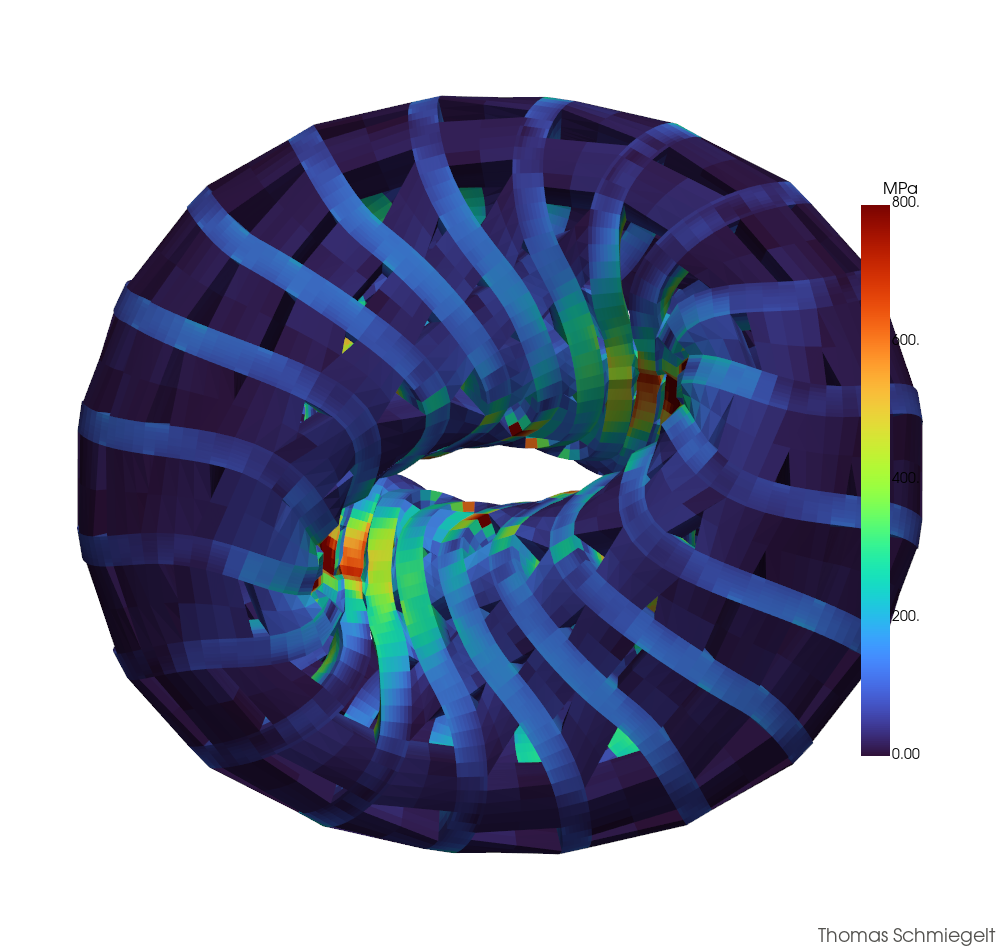
\includegraphics[width=\linewidth]{bilder/spannung_0063.png}\\\footnotesize von Mises stress in the steel (top view, 0–800 MPa)\end{minipage}\hfill
\begin{minipage}[t]{0.49\linewidth}\centering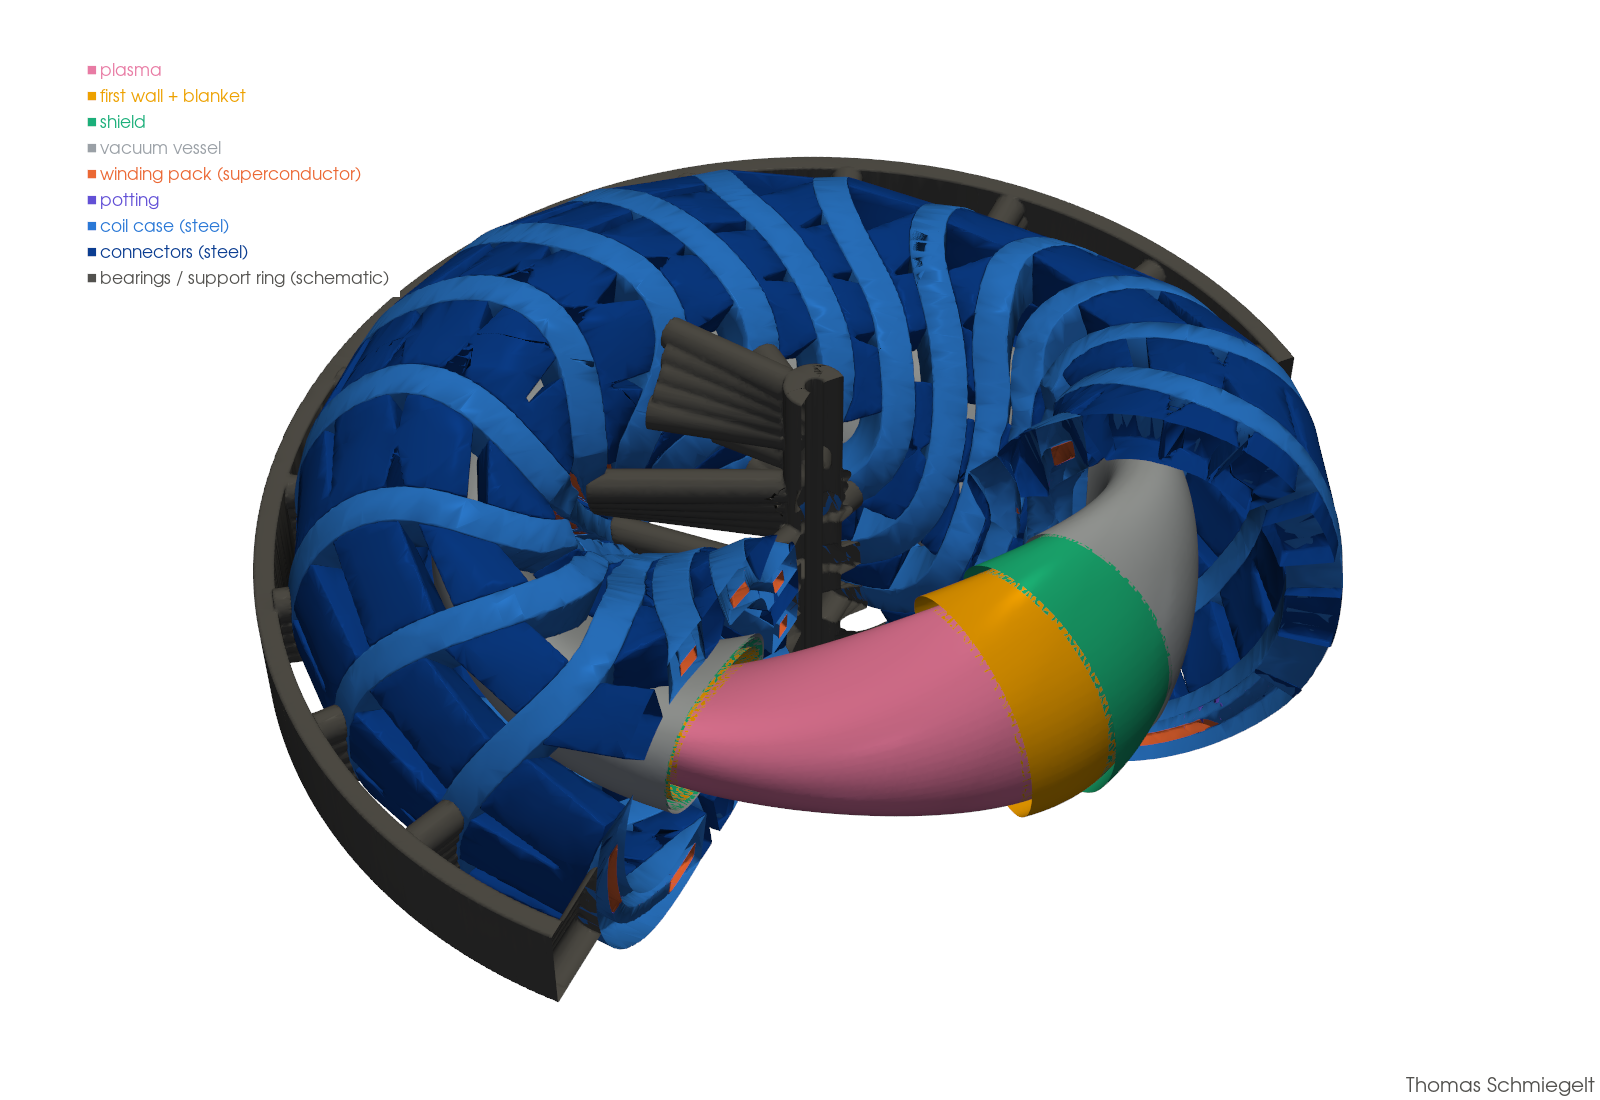
\includegraphics[width=\linewidth]{bilder/modell3d_0063_schnitt_en.png}\\\footnotesize PicoGK model, stepped cut\end{minipage}\hfill
\caption{Design 0063}\end{figure}
\clearpage
\subsection{Design 0136}\label{sb:0136}
\noindent\textbf{Verdict: }Admissible in doe1, no longer with the standard mesh: bottleneck σ99 steel 1.4429 (reserve -15 \%).\par\smallskip
\begin{minipage}[t]{0.46\linewidth}\small\begin{tabular}[t]{@{}lr@{}}\toprule\multicolumn{2}{@{}l}{\textbf{Design variables}}\\\midrule
coil–plasma distance & \num{0.232} \\
coils in total & 20 \\
coils per half period & \num{5} \\
length per coil & \num{4.51} \\
force weight & \num{0.012} \\
inner wall & \num{0.16} \\
side wall & \num{0.30} \\
outer wall min. & \num{0.57} \\
outer wall extra & \num{0.22} \\
connector stiffness & \num{21} \\
connectors per pair & \num{13} \\
bearing radius & \num{3.12} \\
\bottomrule\end{tabular}\end{minipage}\hfill
\begin{minipage}[t]{0.5\linewidth}\small\begin{tabular}[t]{@{}lr@{}}\toprule\multicolumn{2}{@{}l}{\textbf{Results}}\\\midrule
$\sigma_{99}$ steel 1.4429 & \num{577} MPa \\
largest element & \num{2238} MPa \\
$P_m$ max. / 99 \% & \num{2201} / \num{690} MPa \\
$P_m+P_b$ max. & \num{2291} MPa \\
connectors σ99 & \num{141} MPa \\
max. deformation & \num{54} mm \\
winding-pack strain & \num{0.30} \% \\
current per coil & \num{17.7} MA \\
field at conductor & \num{16.9} T \\
utilisation / margin & \num{32} \% / \num{23} K \\
field error $B\cdot n$ & \num{1.62} ‰ \\
clearance plasma–case & \num{1.84} m \\
nuclear heating / fluence & \num{1} W/m³ / 9.6e15 \\
steel case + connectors & \num{10.0} + \num{16.3} kt \\
connectors built & 254 \\
\bottomrule\end{tabular}\end{minipage}\par\medskip
\noindent\textit{Mesh study ($\sigma_{99}$/max. in MPa): }doe1: 479/995; standard: 577/2238.\par\smallskip
\begin{figure}[H]\centering
\begin{minipage}[t]{0.49\linewidth}\centering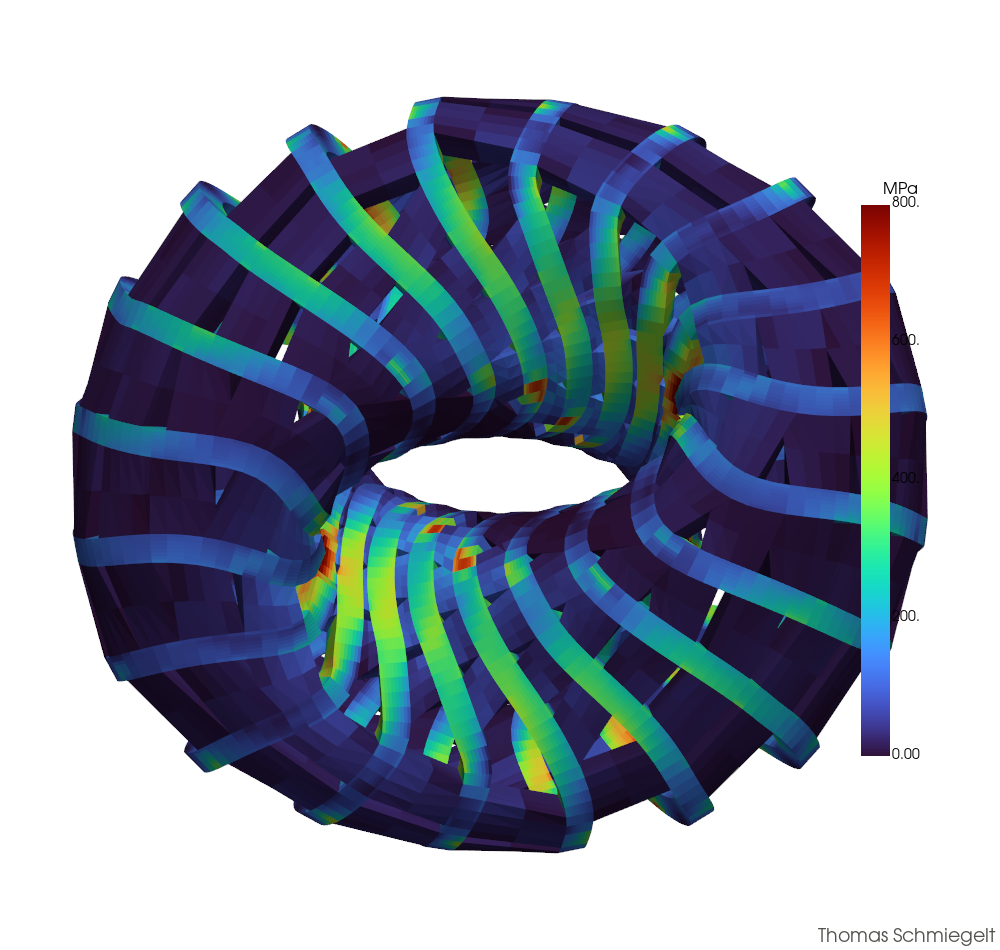
\includegraphics[width=\linewidth]{bilder/spannung_0136.png}\\\footnotesize von Mises stress in the steel (top view, 0–800 MPa)\end{minipage}\hfill
\begin{minipage}[t]{0.49\linewidth}\centering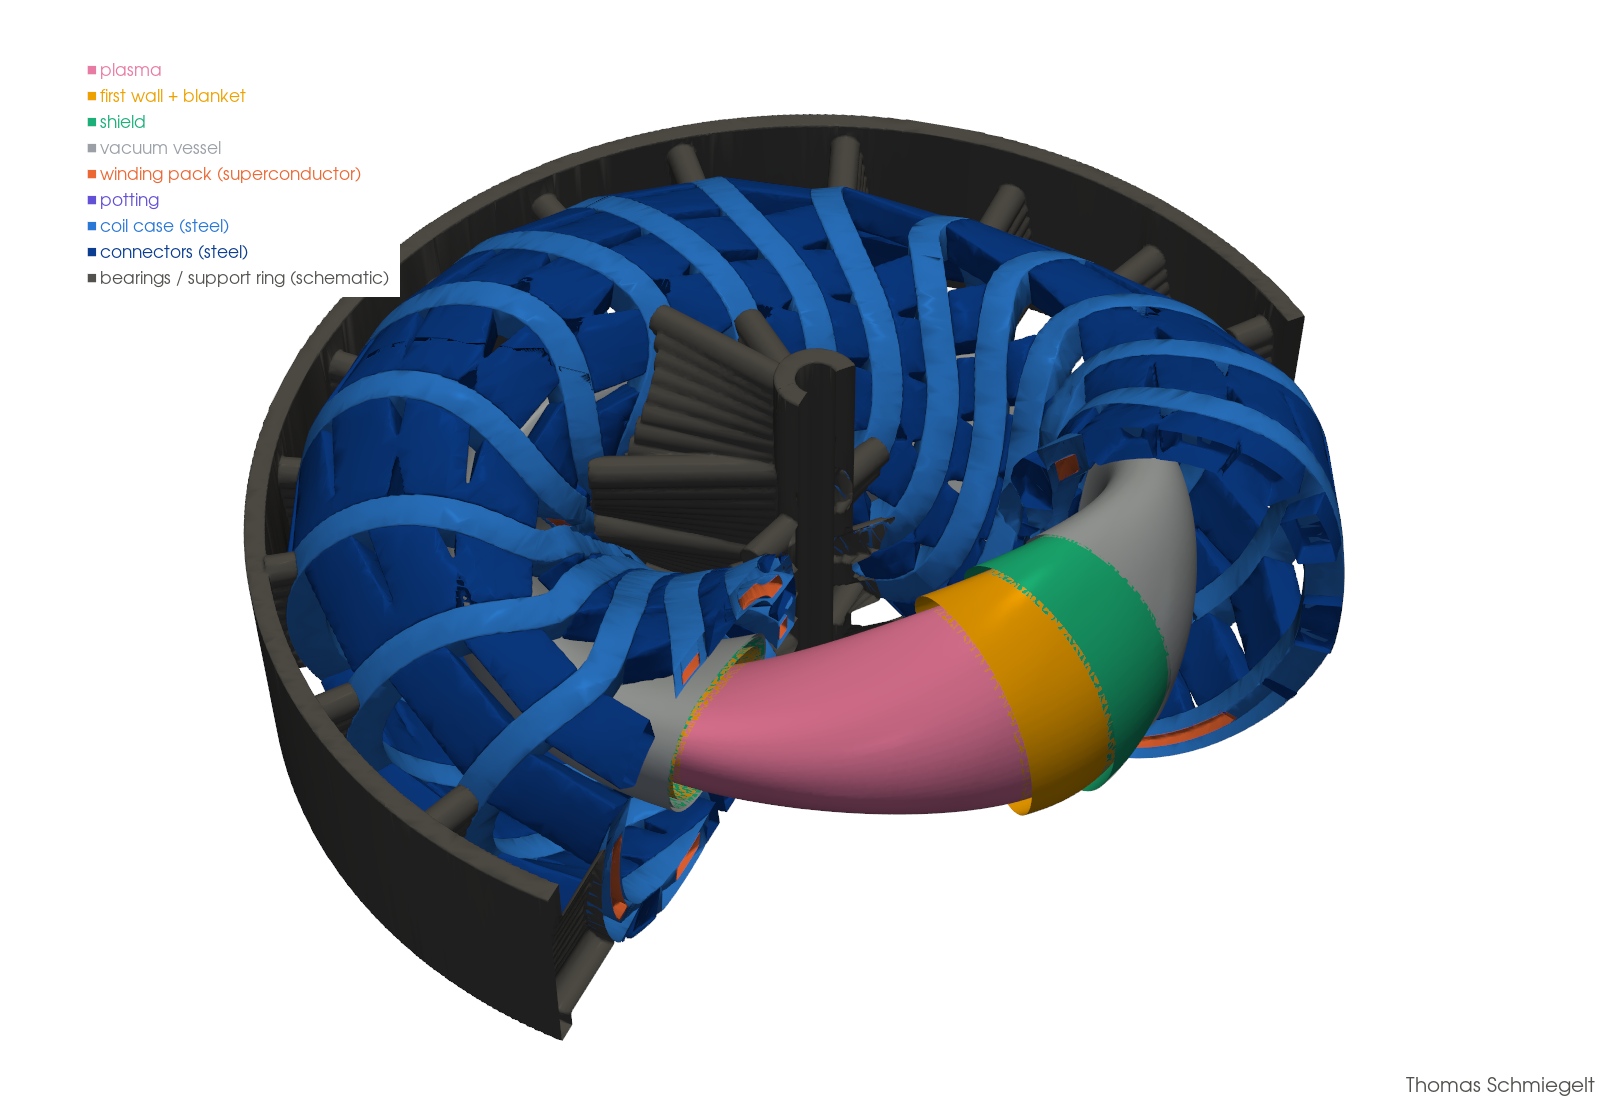
\includegraphics[width=\linewidth]{bilder/modell3d_0136_schnitt_en.png}\\\footnotesize PicoGK model, stepped cut\end{minipage}\hfill
\caption{Design 0136}\end{figure}
\clearpage
\subsection{Surrogate proposal V3}\label{sb:V3}
\noindent\textbf{Verdict: }Surrogate proposal (section~\ref{sec:ersatz1}), admissible; smallest reserve 35 \% (field error B·n).\par\smallskip
\begin{minipage}[t]{0.46\linewidth}\small\begin{tabular}[t]{@{}lr@{}}\toprule\multicolumn{2}{@{}l}{\textbf{Design variables}}\\\midrule
coil–plasma distance & \num{0.205} \\
coils in total & 24 \\
coils per half period & \num{6} \\
length per coil & \num{4.15} \\
force weight & \num{0.022} \\
inner wall & \num{0.20} \\
side wall & \num{0.24} \\
outer wall min. & \num{0.77} \\
outer wall extra & \num{0.48} \\
connector stiffness & \num{176} \\
connectors per pair & \num{11} \\
bearing radius & \num{3.02} \\
\bottomrule\end{tabular}\end{minipage}\hfill
\begin{minipage}[t]{0.5\linewidth}\small\begin{tabular}[t]{@{}lr@{}}\toprule\multicolumn{2}{@{}l}{\textbf{Results}}\\\midrule
$\sigma_{99}$ steel 1.4429 & \num{272} MPa \\
largest element & \num{656} MPa \\
$P_m$ max. / 99 \% & \num{621} / \num{302} MPa \\
$P_m+P_b$ max. & \num{724} MPa \\
connectors σ99 & \num{178} MPa \\
max. deformation & \num{13} mm \\
winding-pack strain & \num{0.13} \% \\
current per coil & \num{14.7} MA \\
field at conductor & \num{15.6} T \\
utilisation / margin & \num{30} \% / \num{24} K \\
field error $B\cdot n$ & \num{1.96} ‰ \\
clearance plasma–case & \num{1.54} m \\
nuclear heating / fluence & \num{22} W/m³ / 1.8e17 \\
steel case + connectors & \num{12.3} + \num{16.8} kt \\
connectors built & 256 \\
\bottomrule\end{tabular}\end{minipage}\par\medskip
\noindent\textit{Mesh study ($\sigma_{99}$/max. in MPa): }standard: 272/656; 1.5× stations: 394/1841.\par\smallskip
\begin{figure}[H]\centering
\begin{minipage}[t]{0.49\linewidth}\centering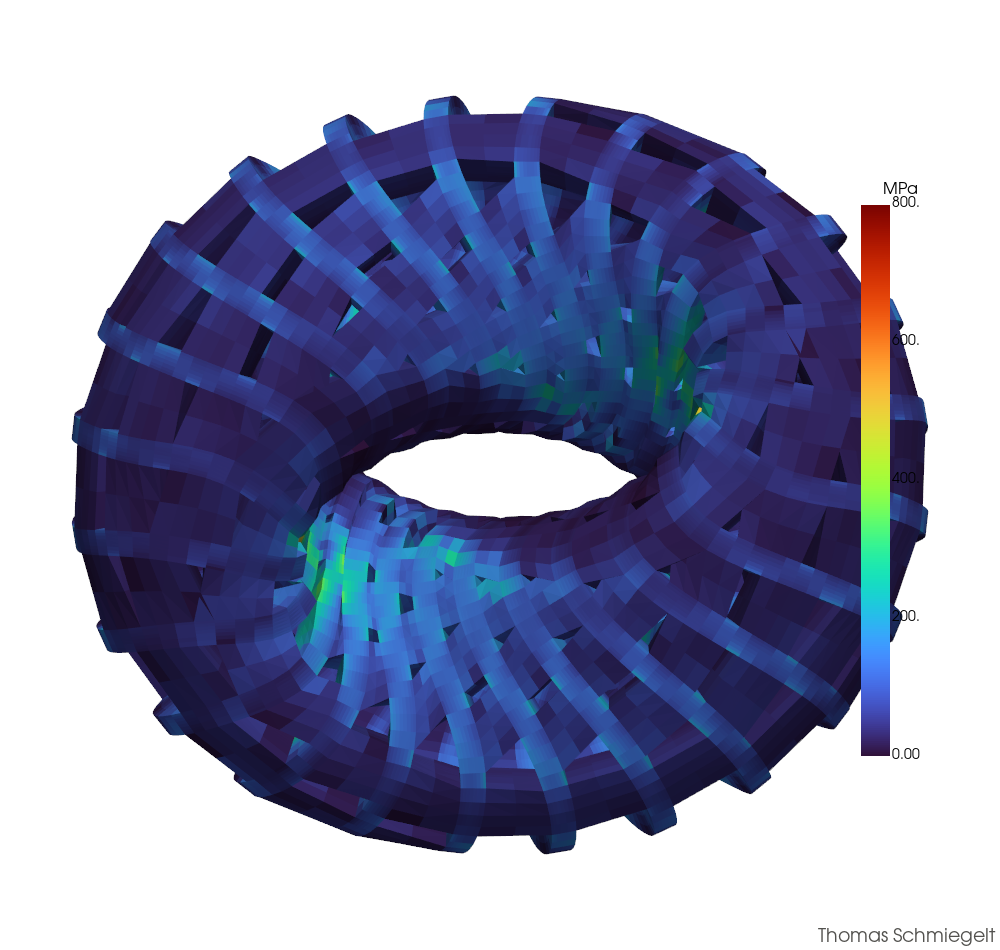
\includegraphics[width=\linewidth]{bilder/spannung_V3.png}\\\footnotesize von Mises stress in the steel (top view, 0–800 MPa)\end{minipage}\hfill
\begin{minipage}[t]{0.49\linewidth}\centering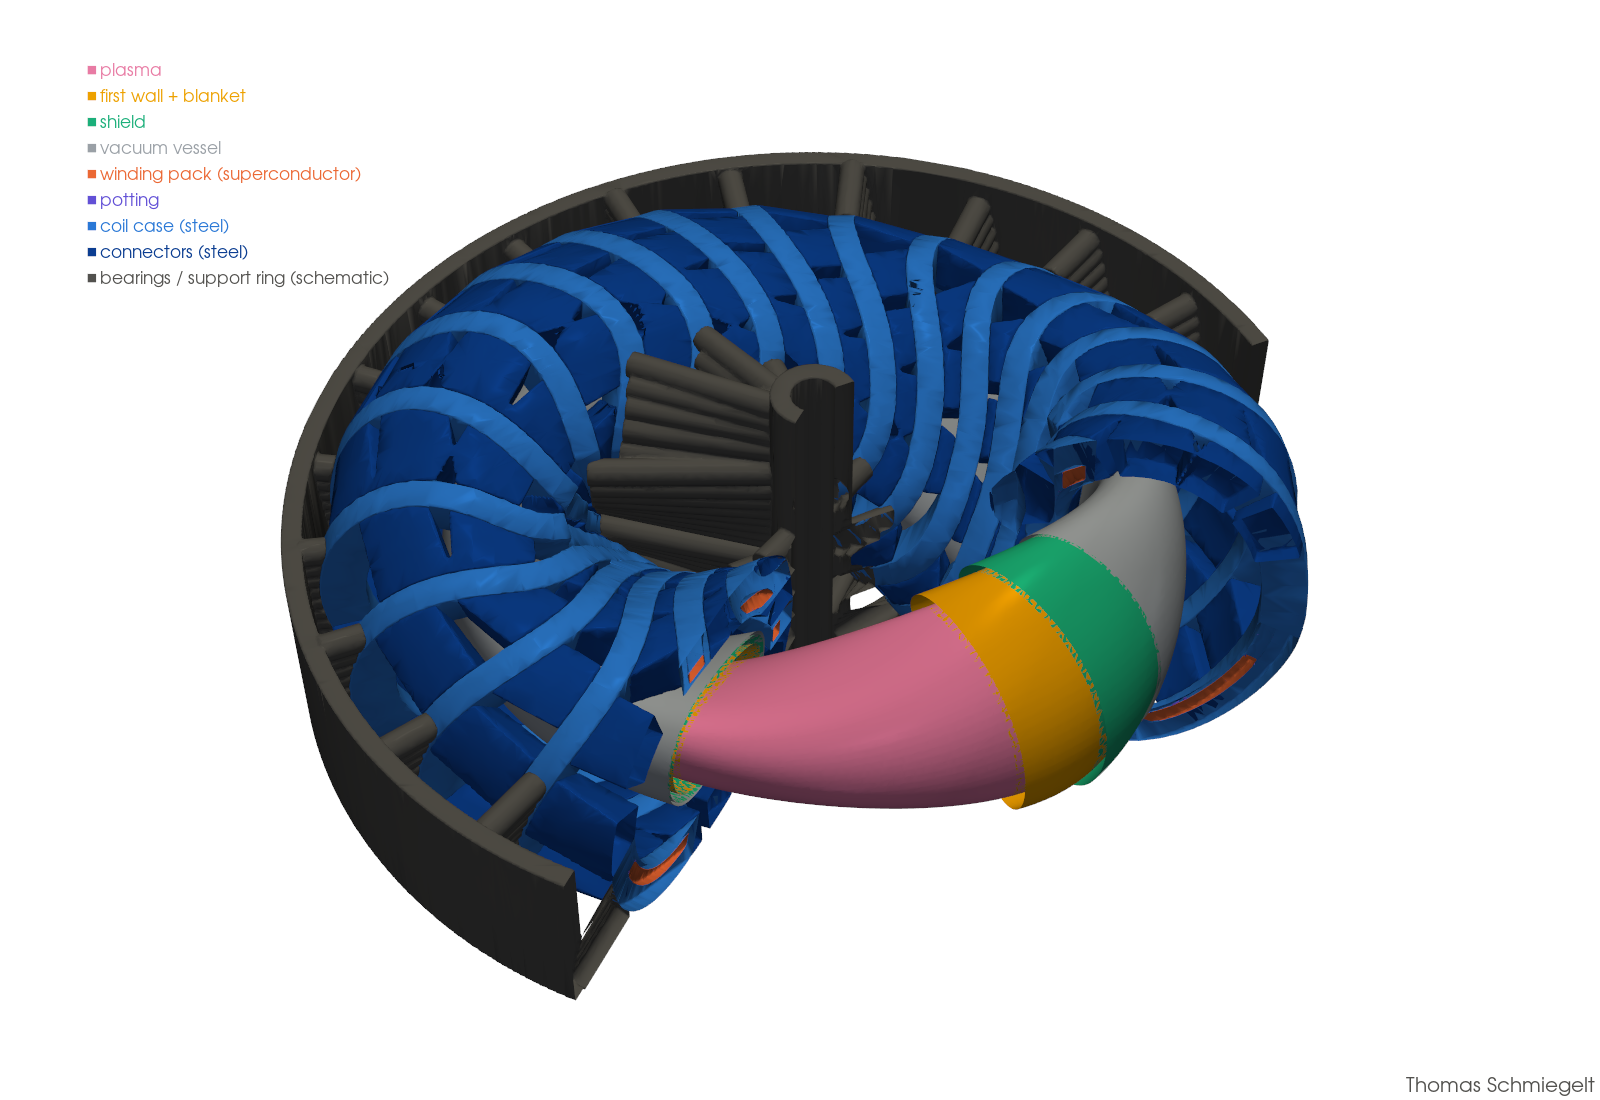
\includegraphics[width=\linewidth]{bilder/modell3d_V3_schnitt_en.png}\\\footnotesize PicoGK model, stepped cut\end{minipage}\hfill
\caption{Surrogate proposal V3}\end{figure}
\clearpage
\subsection{Surrogate proposal V1}\label{sb:V1}
\noindent\textbf{Verdict: }Surrogate proposal (section~\ref{sec:ersatz1}), admissible; smallest reserve 31 \% (package space).\par\smallskip
\begin{minipage}[t]{0.46\linewidth}\small\begin{tabular}[t]{@{}lr@{}}\toprule\multicolumn{2}{@{}l}{\textbf{Design variables}}\\\midrule
coil–plasma distance & \num{0.208} \\
coils in total & 24 \\
coils per half period & \num{6} \\
length per coil & \num{3.98} \\
force weight & \num{0.023} \\
inner wall & \num{0.36} \\
side wall & \num{0.32} \\
outer wall min. & \num{0.77} \\
outer wall extra & \num{0.33} \\
connector stiffness & \num{77} \\
connectors per pair & \num{13} \\
bearing radius & \num{3.41} \\
\bottomrule\end{tabular}\end{minipage}\hfill
\begin{minipage}[t]{0.5\linewidth}\small\begin{tabular}[t]{@{}lr@{}}\toprule\multicolumn{2}{@{}l}{\textbf{Results}}\\\midrule
$\sigma_{99}$ steel 1.4429 & \num{220} MPa \\
largest element & \num{637} MPa \\
$P_m$ max. / 99 \% & \num{532} / \num{248} MPa \\
$P_m+P_b$ max. & \num{746} MPa \\
connectors σ99 & \num{111} MPa \\
max. deformation & \num{11} mm \\
winding-pack strain & \num{0.12} \% \\
current per coil & \num{14.7} MA \\
field at conductor & \num{15.6} T \\
utilisation / margin & \num{30} \% / \num{24} K \\
field error $B\cdot n$ & \num{1.87} ‰ \\
clearance plasma–case & \num{1.41} m \\
nuclear heating / fluence & \num{85} W/m³ / 7.1e17 \\
steel case + connectors & \num{14.6} + \num{18.5} kt \\
connectors built & 308 \\
\bottomrule\end{tabular}\end{minipage}\par\medskip
\noindent\textit{Mesh study ($\sigma_{99}$/max. in MPa): }standard: 220/637; 1.5× stations: 366/2185.\par\smallskip
\begin{figure}[H]\centering
\begin{minipage}[t]{0.49\linewidth}\centering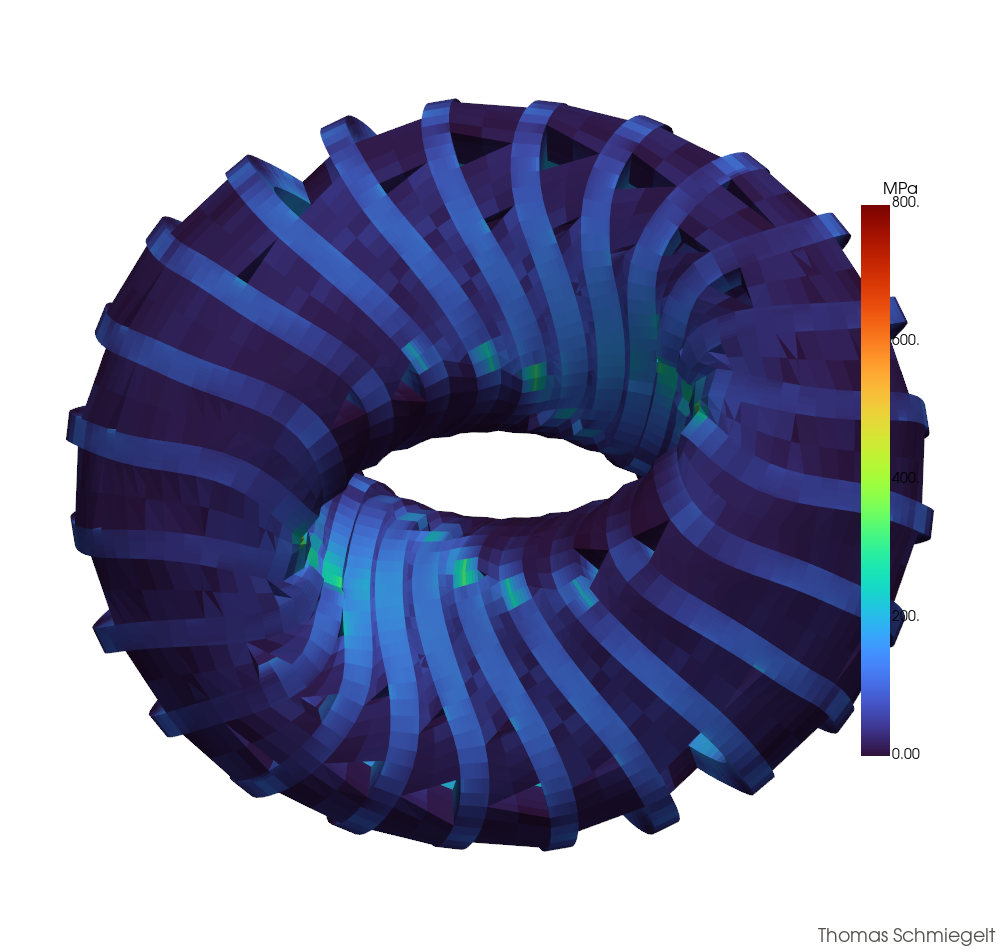
\includegraphics[width=\linewidth]{bilder/spannung_V1.png}\\\footnotesize von Mises stress in the steel (top view, 0–800 MPa)\end{minipage}\hfill
\begin{minipage}[t]{0.49\linewidth}\centering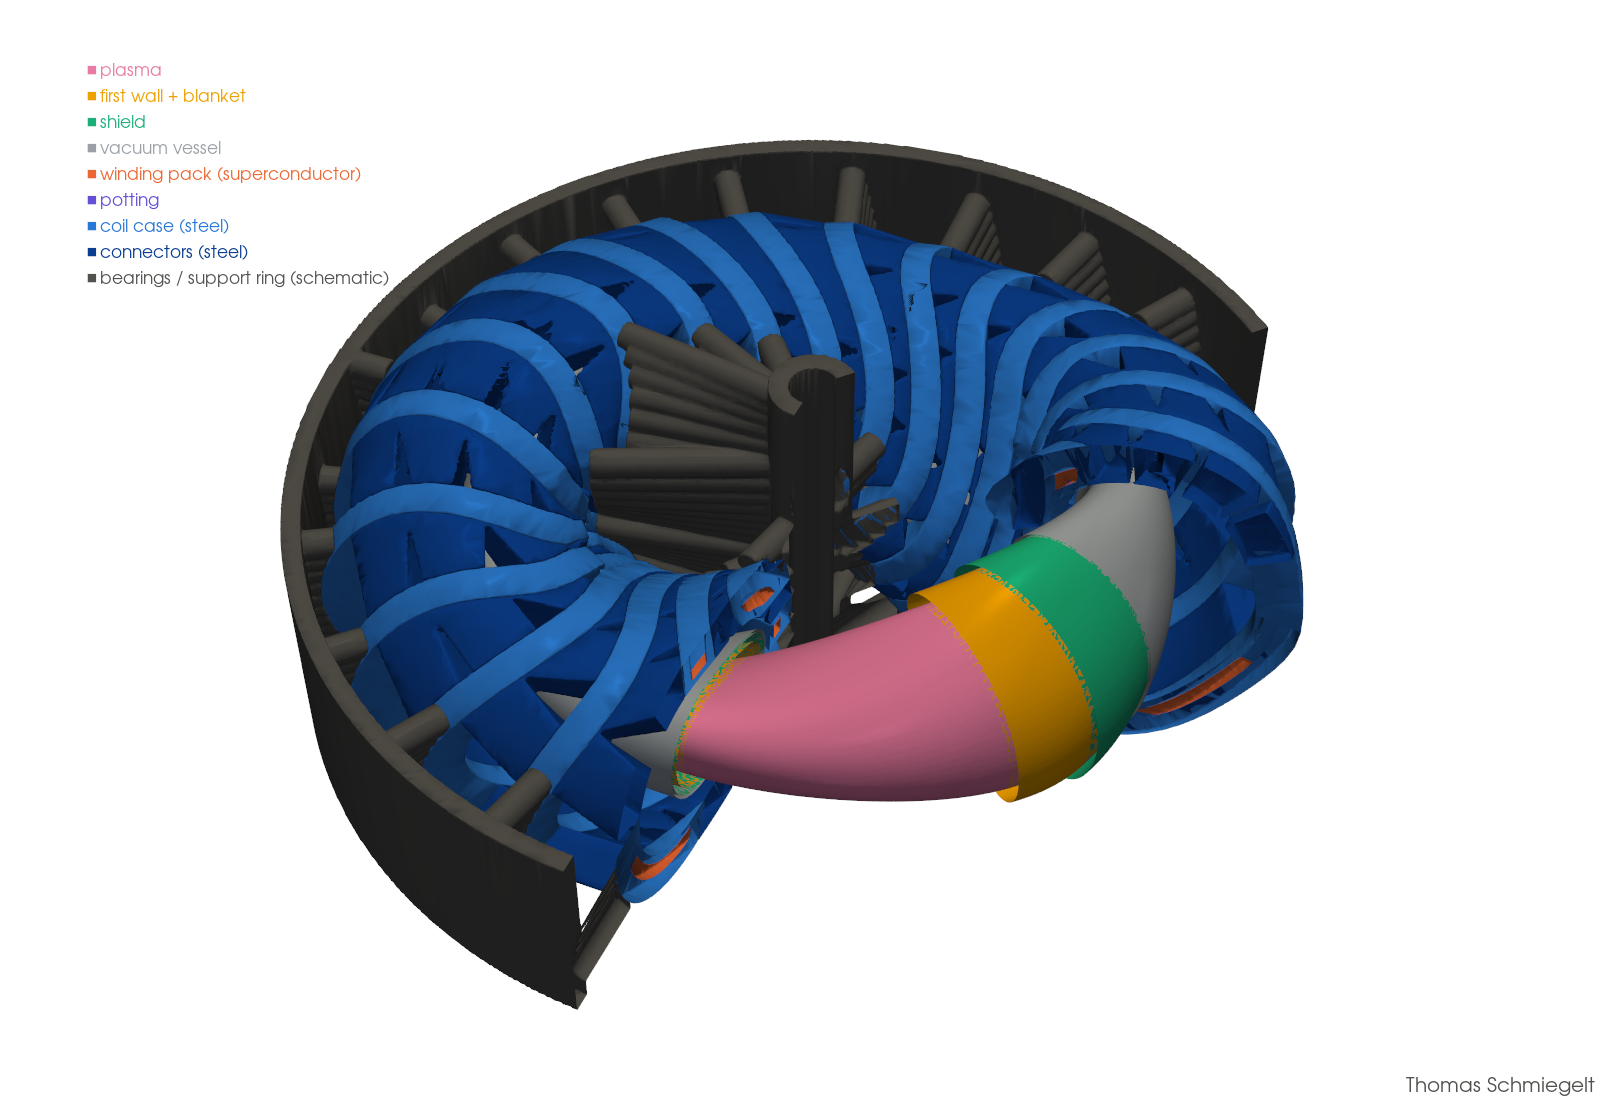
\includegraphics[width=\linewidth]{bilder/modell3d_V1_schnitt_en.png}\\\footnotesize PicoGK model, stepped cut\end{minipage}\hfill
\caption{Surrogate proposal V1}\end{figure}
\clearpage
\subsection{Support test E (thickest walls)}\label{sb:E_test}
\noindent\textbf{Verdict: }Same 16 coils as the starting design; only the support structure differs.\par\smallskip
\begin{minipage}[t]{0.46\linewidth}\small\begin{tabular}[t]{@{}lr@{}}\toprule\multicolumn{2}{@{}l}{\textbf{Design variables}}\\\midrule
coil–plasma distance & \num{0.180} \\
coils in total & 16 \\
coils per half period & \num{4} \\
length per coil & \num{4.50} \\
force weight & \num{0.000} \\
inner wall & \num{0.60} \\
side wall & \num{0.40} \\
outer wall min. & \num{0.80} \\
outer wall extra & \num{0.60} \\
connector stiffness & \num{200} \\
connectors per pair & \num{12} \\
bearing radius & \num{2.50} \\
\bottomrule\end{tabular}\end{minipage}\hfill
\begin{minipage}[t]{0.5\linewidth}\small\begin{tabular}[t]{@{}lr@{}}\toprule\multicolumn{2}{@{}l}{\textbf{Results}}\\\midrule
$\sigma_{99}$ steel 1.4429 & \num{481} MPa \\
largest element & \num{2455} MPa \\
$P_m$ max. / 99 \% & \num{2396} / \num{736} MPa \\
$P_m+P_b$ max. & \num{2515} MPa \\
connectors σ99 & \num{276} MPa \\
max. deformation & \num{41} mm \\
winding-pack strain & \num{0.31} \% \\
current per coil & \num{22.1} MA \\
field at conductor & \num{18.7} T \\
utilisation / margin & \num{34} \% / \num{22} K \\
field error $B\cdot n$ & \num{2.71} ‰ \\
clearance plasma–case & \num{1.53} m \\
nuclear heating / fluence & \num{25} W/m³ / 2.1e17 \\
steel case + connectors & \num{17.6} + \num{19.4} kt \\
connectors built & 168 \\
\bottomrule\end{tabular}\end{minipage}\par\medskip
\begin{figure}[H]\centering
\begin{minipage}[t]{0.49\linewidth}\centering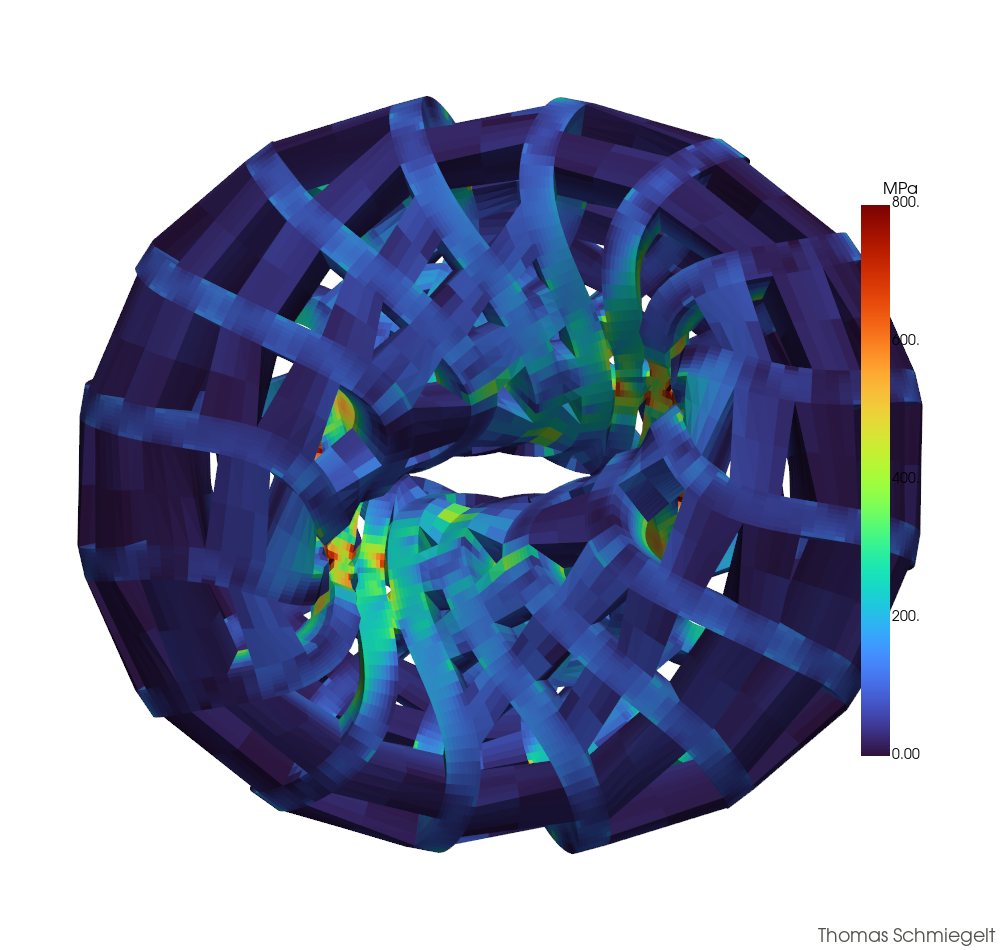
\includegraphics[width=\linewidth]{bilder/spannung_E_test.png}\\\footnotesize von Mises stress in the steel (top view, 0–800 MPa)\end{minipage}\hfill
\begin{minipage}[t]{0.49\linewidth}\centering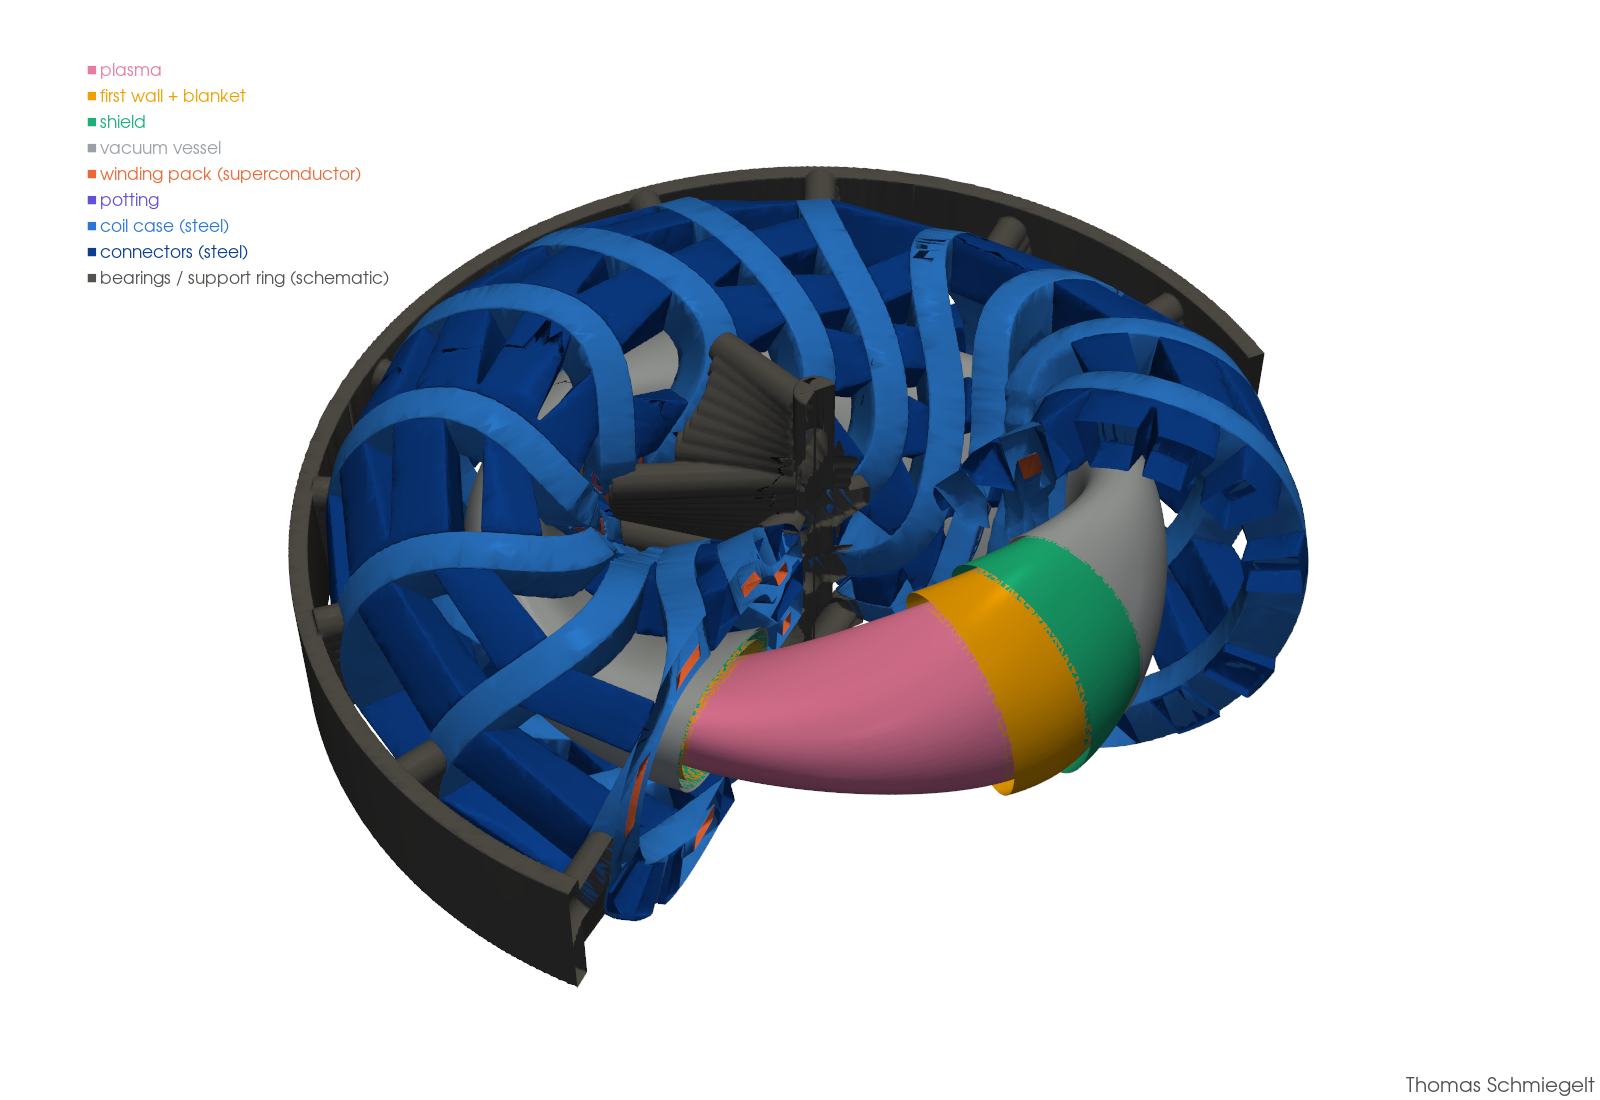
\includegraphics[width=\linewidth]{bilder/modell3d_E_test_schnitt_en.png}\\\footnotesize PicoGK model, stepped cut\end{minipage}\hfill
\caption{Support test E (thickest walls)}\end{figure}
\clearpage
\subsection{Support test A (starting design)}\label{sb:A_test}
\noindent\textbf{Verdict: }Same 16 coils as the starting design; only the support structure differs.\par\smallskip
\begin{minipage}[t]{0.46\linewidth}\small\begin{tabular}[t]{@{}lr@{}}\toprule\multicolumn{2}{@{}l}{\textbf{Design variables}}\\\midrule
coil–plasma distance & \num{0.180} \\
coils in total & 16 \\
coils per half period & \num{4} \\
length per coil & \num{4.50} \\
force weight & \num{0.000} \\
inner wall & \num{0.35} \\
side wall & \num{0.24} \\
outer wall min. & \num{0.45} \\
outer wall extra & \num{0.30} \\
connector stiffness & \num{50} \\
connectors per pair & \num{6} \\
bearing radius & \num{2.50} \\
\bottomrule\end{tabular}\end{minipage}\hfill
\begin{minipage}[t]{0.5\linewidth}\small\begin{tabular}[t]{@{}lr@{}}\toprule\multicolumn{2}{@{}l}{\textbf{Results}}\\\midrule
$\sigma_{99}$ steel 1.4429 & \num{2129} MPa \\
largest element & \num{8454} MPa \\
connectors σ99 & \num{675} MPa \\
max. deformation & \num{399} mm \\
winding-pack strain & \num{0.76} \% \\
current per coil & \num{22.1} MA \\
field at conductor & \num{18.7} T \\
utilisation / margin & \num{34} \% / \num{22} K \\
field error $B\cdot n$ & \num{2.71} ‰ \\
clearance plasma–case & \num{1.77} m \\
nuclear heating / fluence & \num{2} W/m³ / 1.8e16 \\
steel case + connectors & \num{8.5} + \num{7.0} kt \\
connectors built & 90 \\
\bottomrule\end{tabular}\end{minipage}\par\medskip
\begin{figure}[H]\centering
\begin{minipage}[t]{0.49\linewidth}\centering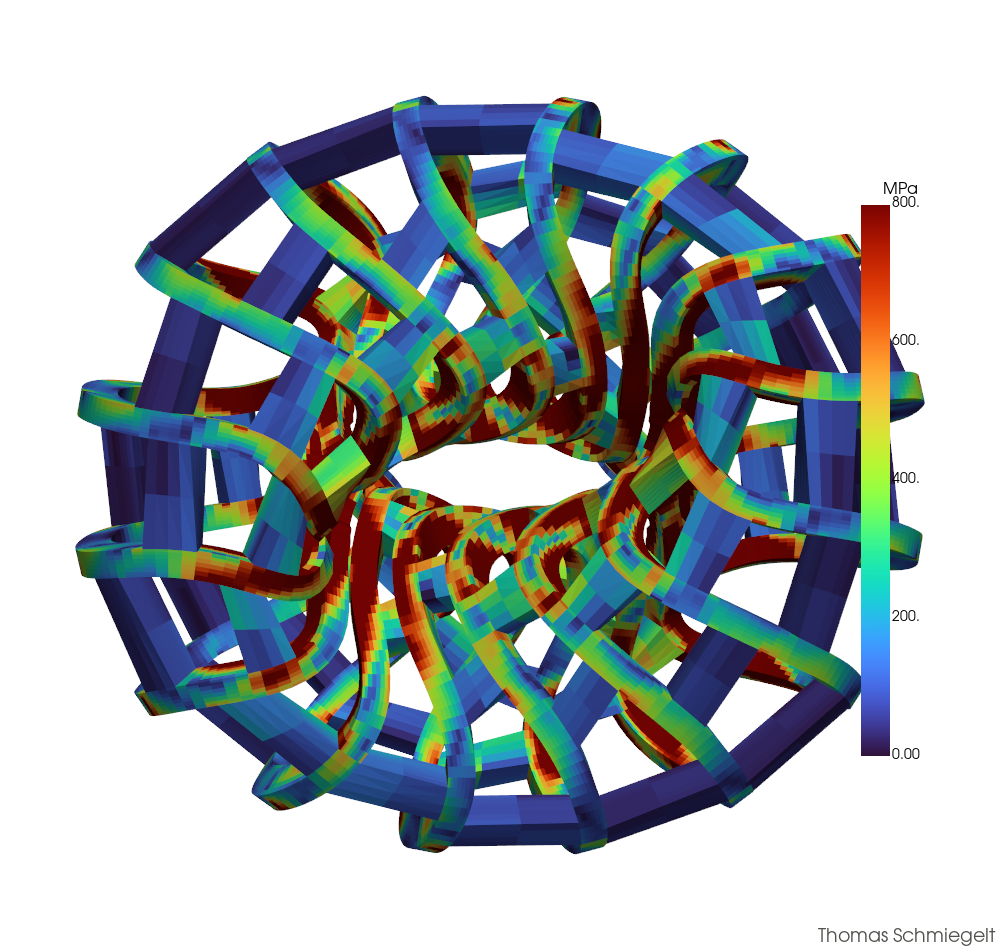
\includegraphics[width=\linewidth]{bilder/spannung_A_test.png}\\\footnotesize von Mises stress in the steel (top view, 0–800 MPa)\end{minipage}\hfill
\begin{minipage}[t]{0.49\linewidth}\centering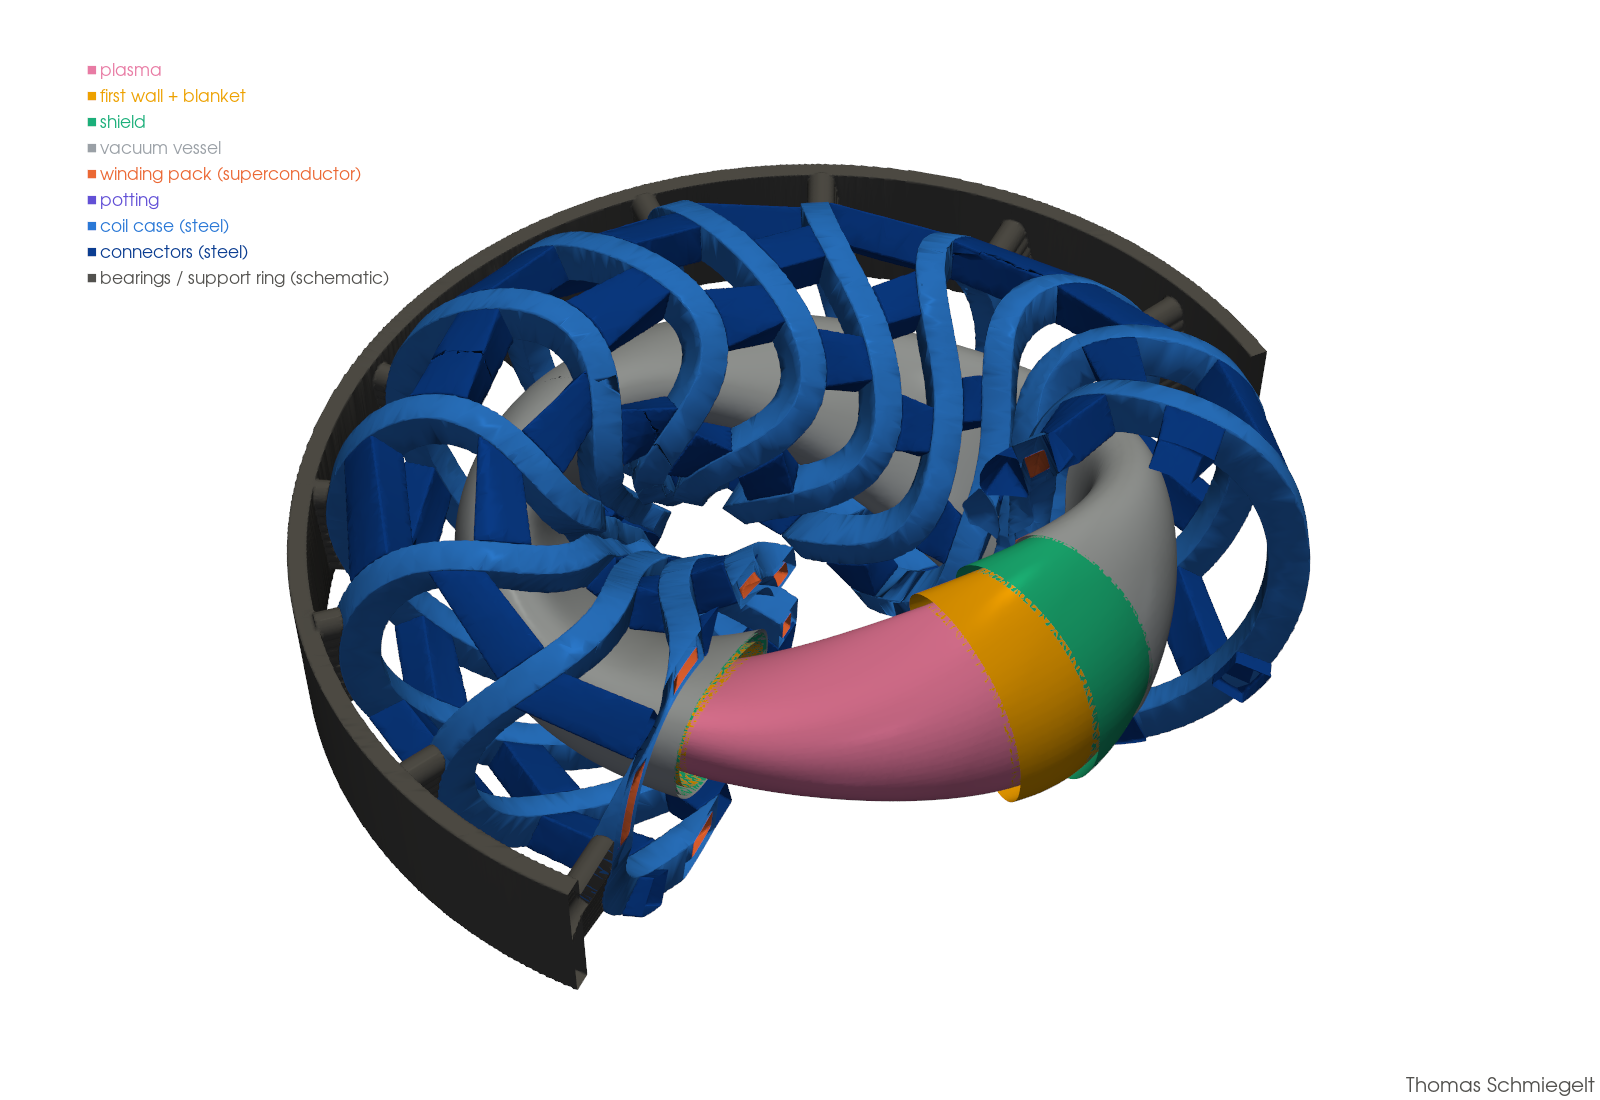
\includegraphics[width=\linewidth]{bilder/modell3d_A_test_schnitt_en.png}\\\footnotesize PicoGK model, stepped cut\end{minipage}\hfill
\caption{Support test A (starting design)}\end{figure}
